\documentclass[a4paper]{article}
\usepackage[utf8]{inputenc}
\usepackage[margin=1in, footskip=0.25in]{geometry}

\usepackage{booktabs}
\usepackage{graphicx}
\graphicspath{../plots}

\usepackage{hyperref}
\usepackage[backend=bibtex, style=numeric, sorting=none]{biblatex}
\bibliography{references}

\usepackage[font=footnotesize,labelfont=bf]{caption}
\captionsetup{width=\linewidth}
\usepackage{subcaption}

\usepackage{listings}
\renewcommand{\lstlistingname}{Code}

\usepackage{xcolor}
\definecolor{backcolour}{RGB}{239,235,230}
\definecolor{lightgray}{gray}{0.7}
\lstdefinestyle{matlabcode}{
	language		=Matlab,
	backgroundcolor	=\color{backcolour},
	basicstyle		=\ttfamily\footnotesize,
	commentstyle	=\color{lightgray},
	numbers			=left,                    
	numbersep		=5pt,
	tabsize			=4,
	showstringspaces=false,
	frame			=leftline,
	captionpos 		= b
}
\lstset{style=matlabcode}

\usepackage{amsmath}
\usepackage{enumitem}


\begin{document}
	
	% ======================= start titlepage ==============================================
	
	\begin{titlepage}
		\begin{center}
			\Large Numerical Methods in Astrophysics \\
			\vspace{1cm}
			\huge{
				Project 3 \\
				\vspace{0.5cm}
				\textbf{Two Dimensional Random Walk,}\\
				\textbf{Circular Binary and} \\
				\textbf{Hypervelocity Stars} \\
				\vspace{1cm}
			}
			\Large \emph{Saksham Kaushal}
		\end{center}
	\end{titlepage}
	
	% =========================end titlepage ================================================
	
	\tableofcontents
	\newpage
	
	% ========================= Problem 1 ===================================================
	
	\part{Two Dimensional Random Walk} \label{problem1}
	
		% ------------------------------- Introduction --------------------------------------
		
		\section{Introduction} \label{1:introduction}
		
		A two dimensional random walk is a process that describes the path of an object in a two dimensional plane consisting of successive random steps. In physics, these processes play an important role in study of polymers, Brownian motion, diffusion, etc. In this problem, such a random walk is visualized. This problem also investigates the number distribution of particles with distance, after a given number of steps in random walks are executed.
		
		% -------------------------------- Methods, Results ---------------------------------
		
		\section{Methods, Results and Discussions} \label{1:methods_results}
		
		\begin{figure} [h]
			\begin{subfigure} {.475\columnwidth}
				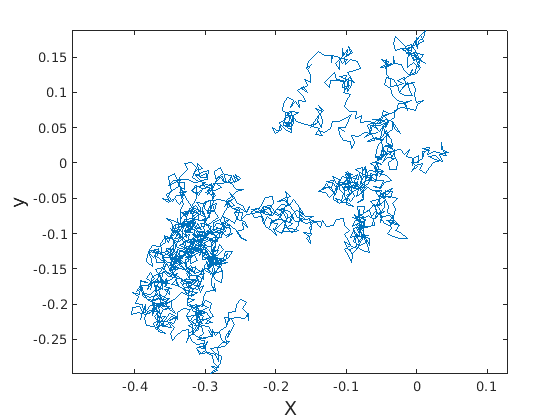
\includegraphics[width=\columnwidth]{../plots/1aa_randomwalk.png}
				\caption{Two dimensional random walk of a particle over 2000 time steps}
				\label{fig:1a}
			\end{subfigure}%
			\hfill
			\begin{subfigure} {.475\columnwidth}
				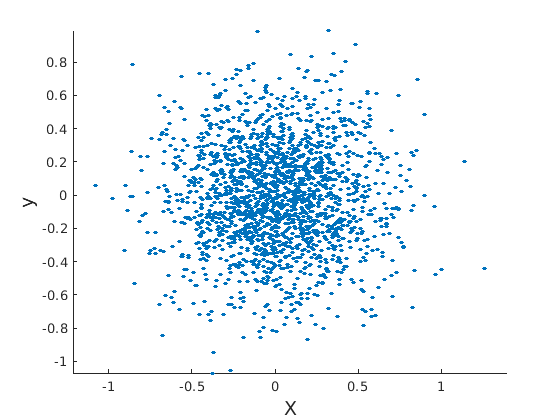
\includegraphics[width=\columnwidth]{../plots/1ab_randomwalk.png}
				\caption{Distribution of final coordinates of 2000 random walk particles}
				\label{fig:1b}
			\end{subfigure}
			
			\begin{subfigure} {.475\columnwidth}
				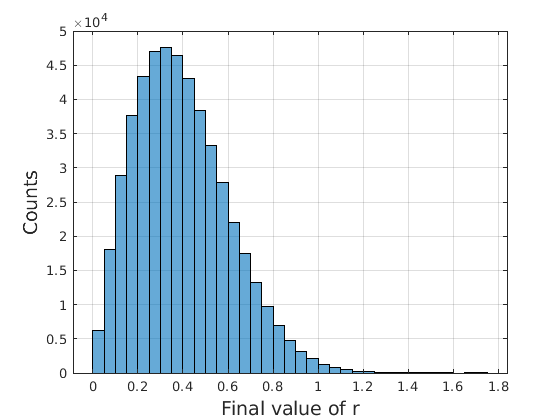
\includegraphics[width=\columnwidth]{../plots/1ac_hist_randomwalk.png}
				\caption{Number distribution with distance of \(5 \times 10^5\) random walk particles}
				\label{fig:1c}
			\end{subfigure}%
			\hfill
			\begin{subfigure} {.475\columnwidth}
				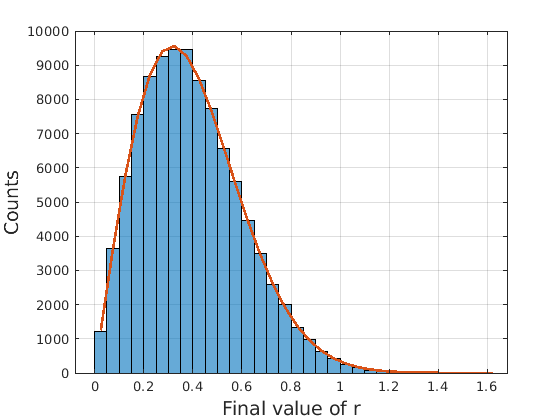
\includegraphics[width=\columnwidth]{../plots/1ad_hist_randomwalk.png}
				\caption{Theoretical estimates and observed distribution of \(10^5\) random walk points. The blue histogram represents the observed number distribution , while the red line is a plot of analytical estimates.}
				\label{fig:1d}
			\end{subfigure}
			\caption{Plotted results for problem 1.1A.}
			\label{fig:1}
		\end{figure}
		
		\begin{enumerate} [label*=\textbf{(\alph*)}]
			
			% ---------------------------------- (a) ---------------------------------------------
			
			\item 
				\subitem \textbf{Methods  --} 
					Random walk of a particle which is initially located at origin (0,0), is computed for 2000 time steps. At each time step, the object moves a distance, \(d=0.01\) units in a random direction which is mathematically represented using angle, \(\theta \in [0,2\pi]\), computed in the Matlab program with the help of inbuilt function, \texttt{rand()}. This function generates random number uniformly in the range \([0,1]\), therefore, multiplying the obtained random number by \(2\pi\) give us the random angle \(\theta\), in line 6 of the code \ref{code:1.1} Successive movements in the two dimensional plane are computed in lines 7 and 8 of code \ref{code:1.1}, which are enclosed in a \emph{for loop} defined in line 5, which repeats the process for each of the 2000 time steps.
					
					\begin{figure} [h]
						\lstinputlisting[caption=prob1aa.m - 2D random walk of a particle, label=code:1.1]{../problem1/prob1aa.m}
					\end{figure}
					
				\subitem \textbf{Results --} 
					The plot of two dimensional random walk of a particle obtained using Matlab code given in code \ref{code:1.1} is shown in figure \ref{fig:1a}.
				
				% \subitem \textbf{Discussion --}
			
			% ---------------------------------- (b) ---------------------------------------------
			
			\item 
				\subitem \textbf{Methods  --} 
					Random walk for 2000 time steps, like the one performed in previous part is performed for 2000 different particles. Accordingly, the crux of code \ref{code:1.1} is executed in a \emph{for loop}, 2000 times, i.e. once for each particle, as shown in line 4 of code \ref{code:1.2}. Instead of visualizing the complete path of random walk, this time only the final coordinates of the particle after finishing the random walk are considered and stored separately in lines 12 and 13 of code \ref{code:1.2}.   
					
					\begin{figure} [h]
						\lstinputlisting[caption=prob1ab.m - Scatter of final positions of 2000 2D random walks, label=code:1.2]{../problem1/prob1ab.m}
					\end{figure}
					
				\subitem \textbf{Results --} 
					A scatter plot of final positions after 2000 time steps, of 2000 particles undergoing two dimensional random walk is shown in figure \ref{fig:1b}. 
				
				% \subitem \textbf{Discussion --}
			
			% ---------------------------------- (c) ---------------------------------------------
			
			\item 
				\subitem \textbf{Methods  --} 
					Using elements from code \ref{code:1.2}, final positions of \(5 \times 10^{5}\) particles are computed. The functions \texttt{tic} and \texttt{toc} are used to compute the time elapsed in execution of the code. With the help of these functions, the total number of particles is chosen, based purely on estimate of the maximum computations that can be performed in feasible time. So, The initial 18 lines of code \ref{code:1.3} are essentially adopted from code \ref{code:1.2}, with an exception of line 17, where the modulus of displacement of a particle from origin is calculated. The following lines evaluate and plot the histogram of number distribution of particles with distance travelled. Using a bin width of \(dr=0.05\), binedges are computed and the histogram is plotted on line 24.\\
					An alternate method in which counts in each bin are calculated to produce the histogram, was used to confirm results, and is not shown in code \ref{code:1.3}. 
					
					\begin{figure} [h]
						\lstinputlisting[caption=prob1ac.m - Number distribution with distance of \(5 \times 10^5\) particles, label=code:1.3]{../problem1/prob1ac.m}
					\end{figure}
					
				\subitem \textbf{Results --}
					The histogram showing particle number distribution, \(N(r,r+\Delta r)\), of 500000 particles for \(\Delta r = 0.05\) is given in figure \ref{fig:1c}. 
				
				%\subitem \textbf{Discussion --}
				
			% ---------------------------------- (d) ---------------------------------------------
			
			\item 
				\subitem \textbf{Methods  --} 
					Initial lines of code \ref{code:1.4}, till line 27, are adopted from code \ref{code:1.3} and the value of \texttt{np} is set to \(10^5\), i.e. histogram is generated for \(10^5\) particles. Theoretically expected number distribution is then computed for each bin in lines 30-33, and the obtained curve is overlayed on the histogram. Analytically calculated number distribution of particles with distance is given by equation (3) of project notes as,
					\begin{equation}
						N(r,r+\Delta r) = N^{}_{p} \exp\left( -\frac{r^2_{}}{nd^2_{}} \right) \left\lbrace 1- \exp \left( - \frac{\Delta r (2r+\Delta r)}{nd^2_{}} \right) \right\rbrace ,
						\label{eq:number_distribution}
					\end{equation}
					where, \(N(r,r+\Delta r)\) is the number of particles that have eventually travelled an absolute value of displacement in the range \([r,r+\Delta r]\), \(N_p^{}\) is the total number of particles, \(n\) is the number of time steps and \(d\) is the jump size at each time step. This equation \ref{eq:number_distribution} is encoded in code \ref{code:1.4} in lines 31 and 32.
					\begin{figure} [h]
						\lstinputlisting[caption=(Part of) prob1ad.m - Analytical estimates and observed 	number distributions with distance of \(10^5\) particles, 
										label=code:1.4, firstline=28, firstnumber=28,
										lastline=35]{../problem1/prob1ad.m}
					\end{figure}
					
				\subitem \textbf{Results --} 
					The histogram for \(10^5\) particles is shown in figure \ref{fig:1d}. The analytical estimates is overlayed on the same plot. 
				
				\subitem \textbf{Discussion --}
					For a large number of particles, the observed number distribution seems to coincide well with the theoretical estimates, as seen in figure \ref{fig:1d}.
				
			% ---------------------------------- (e) ---------------------------------------------
			
			\item
				\subitem \textbf{Methods --}
					The number distribution of photons in this case is given by,
					\begin{equation}
						N(r) dr = 2 \pi r \rho (r) dr,
						\label{eq:photon_num_distribution}
					\end{equation}
					where, \(\rho (r)\) is the particle density distribution, given by,
					\begin{equation}
						\rho (r) = \frac{N_p^{}}{\pi n d^2_{}} \exp \left( - \frac{r^2_{}}{nd^2_{}} \right)
						\label{eq:photon_particle_density} 
					\end{equation}
					Substituting equation \ref{eq:photon_particle_density} in equation \ref{eq:photon_num_distribution}, we obtain,
					\[N(r)dr = \frac{2rN_p^{}}{nd^2_{}} \exp \left( - \frac{r^2_{}}{nd^2_{}} \right) dr.\]
					At peak number density, derivative of \(n\) with respect to displacement \(r\) equals zero. From this we obtain,
					\[\frac{dN}{dr} = \frac{2N_p^{}}{nd^2_{}} \frac{d}{dr} \left[ r \exp \left( - \frac{r^2_{}}{nd^2_{}} \right) \right] = 0 \]
					\[\Rightarrow \frac{2N_p}{nd^2_{}} \exp \left( - \frac{r^2_{}}{nd^2_{}} \right) \left[ 1- \frac{2r^2_{}}{nd^2_{}} \right] = 0 \]
					
					\begin{equation}
						\Rightarrow n = \frac{2r^2_{}}{d^2_{}}
						\label{eq:num_distribution_deriv1}
					\end{equation}
					
					Using value of \(r = R_\odot^{} = 7 \times 10^8_{}\) m and \(d=1\) mm \(=10^{-3}_{}\) m in equation \ref{eq:num_distribution_deriv1}, we get, number of time steps,
					
					\begin{equation}
						n = 9.8 \times 10^{23}_{}.
						\label{eq:num_distribution_value}
					\end{equation}
					
					Total distance travelled by the photon before reaching the surface is, \(s = \) number of time steps \(\times\) distance travelled in each time step, i.e.,
					
					\begin{equation}
						s = 9.8\times 10^{23}_{} \times 10^{-3} = 9.8 \times 10^{20} \text{m}.
					\end{equation}
					
					With photon travelling at speed of light, \(c\), the time elapsed is given by,
					
					\begin{equation}
					 	t = \frac{s}{c} \approx 3.267 \times 10^{12}_{} \text{sec} \approx 10^5 \text{years}
					 	\label{eq:final_t_estimate}
					\end{equation}
					
				\subitem \textbf{Discussion --}
					The rough estimate of time taken by photon considers an ideal case with several approximations. Despite that, the calculation gives us a reasonable order of magnitude estimate in equation \ref{eq:final_t_estimate}, which is quite close to the value of a few million years, usually obtained for a realistic case.
			
		\end{enumerate}

		% -------------------------------- Conclusions ------------------------------------------
		
		\section{Conclusions} \label{1:conclusions}
		
		For a large sample of random walk data, the number distribution of particles with eventual distance is given by equation \ref{eq:number_distribution}. The theoretical estimates and observations made using numerical simulation seem to agree well. One example of an approximate random walk is the motion of a photon through the layers of Sun. This causes the photon to take several years (of the order of millions) to reach the surface of the Sun before eventually escaping.  
		

	
	% ========================= Problem 2 ===================================================
	
%	\clearpage
	\setcounter{section}{0}
	\part{Circular Binary} \label{Problem2}
	
		% ------------------------------- Introduction --------------------------------------

		\section{Introduction} \label{2:introduction}
		A system of two stars rotating in circular orbits around their common centre of mass is called a \emph{circular binary}. The heavier star is called the primary star whereas the lighter one is called the secondary star. The orbital time period for both the stars is equal and therefore, primary star traverses a small orbit at slower velocity, while the orbit of the secondary star is larger which it traverses at a higher velocity. In most of the commonly encountered systems, evolutionary correlation between the two stars is extremely significant. Such a gravitationally bound system possesses a negative total energy.

		% -------------------------------- Methods, Results ----------------------------------
		
		\section{Methods, Results and Discussions}
	
		\begin{enumerate} [label*=\textbf{(\alph*)}]
			
			% ---------------------------------- (a) ---------------------------------------------
			
			\item
				\subitem \textbf{Methods  --}
				The dimensionless masses and positions of primary and secondary stars are respectively given by,
				\begin{equation}
					\begin{gathered}
						\tilde{m}_p^{}=\frac{m_p^{}}{m} \text{ and } \tilde{m}_s^{}=\frac{m_s^{}}{m}, \\
						\tilde{x}_p^{}=\frac{x_p^{}}{a}, \text{ and } \tilde{x}_s^{}=\frac{x_s^{}}{a},
					\end{gathered}
					\label{eq:dimensionless_mass_pos}
				\end{equation}
				where, \(m\) and \(a\) are the total mass and separation of binary respectively. For a circular binary, the gravitational force experienced by each star equals the centripetal force on the star. Mathematically,
				\begin{equation}
					\begin{gathered}
						\frac{Gm_{s}^{}m_{p}^{}}{a^2_{}} = m_p^{} x_p^{} \omega^2_{} = m_s^{} x_s^{} \omega^2_{} , \\
						\Rightarrow x_s^{} = \frac{x_p^{} m_p^{}}{m_s^{}}.
					\end{gathered}
					\label{eq:secondary_pos}
				\end{equation}
				Total separation of binary is the sum of positions of primary and secondary stars with respect to their centre of mass, \textit{i.e.} 
				\begin{equation}
					x_p^{}+x_s^{} = a.
					\label{eq:binary_separation}
				\end{equation}
				Using equations \ref{eq:secondary_pos} and \ref{eq:binary_separation}, we obtain,
				\begin{equation}
					\begin{gathered}
						x_p + \frac{x_p m_p}{m_s} = a \\
						\Rightarrow x_p \left( \frac{m}{m_s}\right) = a \\
						\Rightarrow \tilde{x}_p = \tilde{m}_s 
					\end{gathered}
					\label{eq:xp_tilde}
				\end{equation}
				This relation gives us the relation for dimensionless position of primary star. Similarly, we can also obtain the relation for dimensionless position of secondary star as,
				\begin{equation}
					\begin{gathered}
						x_s + \frac{x_s m_s}{m_p} = a \\
						\Rightarrow \tilde{x}_s = \tilde{m}_p
					\end{gathered}
					\label{eq:xs_tilde}
				\end{equation}
				
				If we substitute the value of angular velocity, \(\omega =  v_p/r_p = v_s/r_s\), in equation \ref{eq:secondary_pos} for the two stars, we get,
				\begin{equation}
					\begin{gathered}
						\frac{G m_s m_p}{a^2} = \frac{m_p v_p^2}{x_p} = \frac{m_s v_s^2}{x_s} \\
						\Rightarrow \frac{v_p}{v_s} = \frac{m_s}{m_p}
					\end{gathered}
					\label{eq:gravity_centripetal}
				\end{equation}
				Multiplying both numerator and denominator of RHS by \(1/m\), we obtain,
				\begin{equation}
					\frac{v_p}{v_s} = \frac{\tilde{m}_s}{\tilde{m}_p}
					\label{eq:velocity_mass_relation}
				\end{equation}
				
				If we use the first relation of equation \ref{eq:gravity_centripetal}, we get,
				\begin{equation}
					\begin{gathered}
						\frac{G m_s m_p}{a^2} = \frac{m_p v_p^2}{x_p} \\
						\Rightarrow v_p^2 = \frac{G m_s x_p}{a^2} \\
						\Rightarrow v_p^2 = \frac{Gm}{a} \tilde{m}_s \tilde{x}_p = \frac{Gm}{a} \tilde{m}_s^2,
					\end{gathered}
				\end{equation}
				where, we have substituted values from equation set \ref{eq:dimensionless_mass_pos} and equation \ref{eq:xp_tilde}. In units of \(\sqrt{Gm/a}\), we obtain the value of dimensionless velocity of primary star as,
					\begin{equation}
						\tilde{v}_p = \tilde{m}_s
						\label{eq:primary_velocity}
					\end{equation}
				By using equations \ref{eq:gravity_centripetal} and \ref{eq:primary_velocity}, we get dimensionless velocity of secondary as,
					\begin{equation}
						\tilde{v}_s = \tilde{m}_p
						\label{eq:secondary_velocity}
					\end{equation}
				
				Given that angular velocity \(\omega = 2\pi / T\), where \(T\) is the period of the circular binary, we can find the dimensionless time by using equation \ref{eq:secondary_pos}, as,
				\begin{equation}
					\begin{gathered}
						\nonumber \frac{G m_s m_p}{a^2} = m_p x_p \omega^2 \\
						\Rightarrow \frac{G m_s}{a^2} = \frac{4 \pi^2 x_p}{T^2} \\
					\end{gathered}
				\end{equation}
				Using equations \ref{eq:dimensionless_mass_pos} and \ref{eq:xp_tilde}, we get,
				\begin{equation}
					\begin{gathered}
						\frac{G m_s}{a^3} = \frac{4 \pi^2 m_s}{T^2 m} \\
						\Rightarrow T = 2 \pi \sqrt{\frac{a^3}{Gm}}.
					\end{gathered}
				\end{equation}
				In units of \(\sqrt{a^3/Gm}\), we therefore derive dimensionless time of a circular binary as,
				\begin{equation}
					\tilde{T} = 2 \pi
					\label{eq:dimensionless_time}
				\end{equation}
				
				\subitem \textbf{Results  --}
				In the given scenario, the stars lie in x-y plane, with their centre of mass at origin. Primary star has initial coordinates \((-x_{px},0)\) while the secondary stars lies initially at \((x_{py},0)\).\\
				The stars rotate counter-clockwise, which gives us the velocity of primary star, \(-v_{py}\) and the velocity of secondary star, \(v_{sy}\).
				Using equations \ref{eq:xp_tilde}, \ref{eq:xs_tilde}, \ref{eq:primary_velocity} and \ref{eq:secondary_velocity}, the dimensionless values of initial conditions of the stars are summarized in table \ref{table:2_initial_conditions}.\\ The value of dimensionless time period of binary is derived in equation \ref{eq:dimensionless_time} as \(2 \pi\).
				
				\begin{table}
					\centering
					\begin{tabular} {c c c c}
						\toprule
						\textbf{Parameter} & \textbf{Value} & \textbf{Parameter} & \textbf{Value} \\
						(Primary Star) & & (Secondary star) & \\
						\midrule
						\(\tilde{x}_{px}\) & \(-\tilde{m}_s\) & \(\tilde{x}_{sx}\) & \(\tilde{m}_p\) \\
						\(\tilde{x}_{py}\) & 0 & \(\tilde{x}_{sy}\) & 0\\
						\(\tilde{v}_{px}\) & 0 & \(\tilde{v}_{sx}\) & 0 \\
						\(\tilde{v}_{py}\) & \(-\tilde{m}_s\) & \(\tilde{v}_{sy}\) & \(\tilde{m}_p\) \\
						\bottomrule
					\end{tabular}
				\caption{A summary of initial conditions for the simulation. All quantities are mentioned in dimensionless units, for a binary in x-y plane rotating counter-clockwise, with centre of mass at origin and primary star on the negative x-axis and secondary star on positive x-axis initially.}
				\label{table:2_initial_conditions}
				\end{table}
				
				%\subitem \textbf{Discussions  --}
				
			% ---------------------------------- (b) ---------------------------------------------
			
			\item
				\subitem \textbf{Methods  --}
				Given that,
				\begin{equation}
					\frac{m_p}{m_s} = 4
					\label{eq:masses_ratio}
				\end{equation}
				Adding 1 on both side, we get,
				\begin{equation}
					\begin{gathered}
						\nonumber \frac{m_p}{m_s} + 1 = 5 \\
						\Rightarrow \frac{m_p+m_s}{m_s} = \frac{m}{m_s} = 5
					\end{gathered}
				\end{equation}
				\begin{equation}
					\Rightarrow \tilde{m}_s = \frac{m_s}{m} = \frac{1}{5} = 0.2
					\label{eq:secondary_dimensionless_mass}
				\end{equation}
				
				Using equations \ref{eq:dimensionless_mass_pos}, \ref{eq:masses_ratio} and \ref{eq:secondary_dimensionless_mass}, we can obtain the dimensionless mass of primary star as,
				\begin{equation}
					\tilde{m_p} = 4 \times \tilde{m_s} = 0.8
					\label{eq:primary_dimensionless_mass}
				\end{equation} 
				
				\subitem \textbf{Results  --}
				Using relations mentioned in table \ref{table:2_initial_conditions}, the initial conditions for the circular binary are defined in Matlab file \textit{binary.m} a shown in lines 13--20 of code \ref{code:2.1}. Using equations \ref{eq:secondary_dimensionless_mass} and \ref{eq:primary_dimensionless_mass}, the values of dimensionless masses of two stars are assigned in lines 11 and 12 as \texttt{mp = 0.8} and \texttt{ms = 0.2}.\\				
				The value of \texttt{tmax} is set ot \(10\pi\). Since from equation \ref{eq:dimensionless_time}, it is known that the value of dimensionless time is \(2\pi\), this given value of \texttt{tmax} will allow simulation to sun for 5 orbits of the binary. 
				
				\begin{figure} [h] 
					\lstinputlisting[caption=binary.m - Initial conditions of circularly rotating binary for a simulation of five orbital rotations., label=code:2.1,
					firstline=7,firstnumber=9,
					lastline=19]{../problem2/binary.m}
				\end{figure}
				
%				\subitem \textbf{Discussions  --}
			
			\begin{figure} [h]
				\begin{subfigure} {.475\columnwidth}
					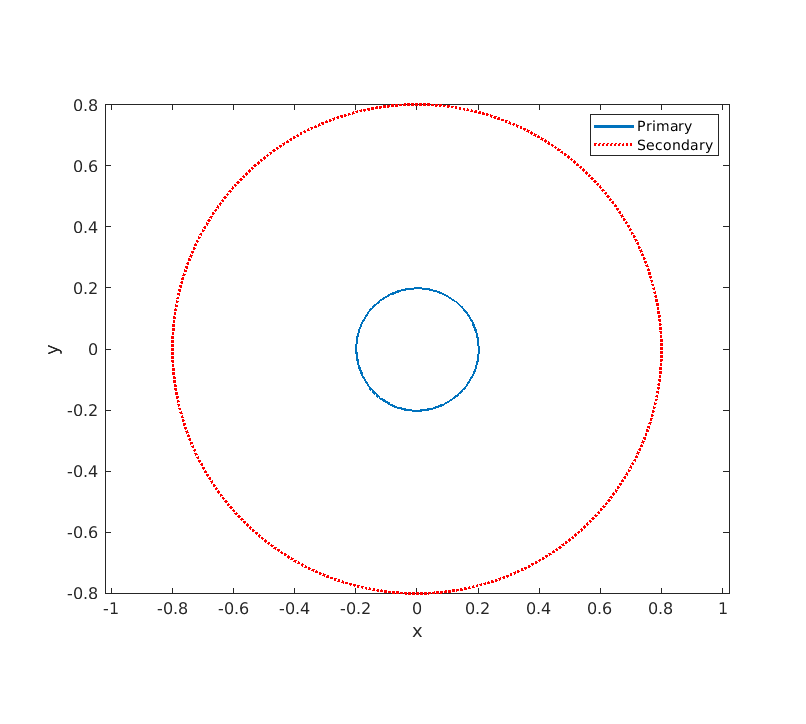
\includegraphics[width=\columnwidth]{../plots/2c_orbits.png}
					\caption{Trajectories of primary and secondary stars in a circular binary system over the first five rotations.}
					\label{fig:2c}
				\end{subfigure}
				\hfill
				\begin{subfigure} {.485\columnwidth}
					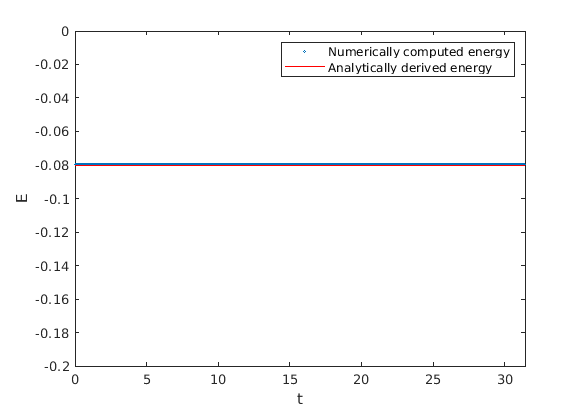
\includegraphics[width=\columnwidth]{../plots/2d_energies.png}
					\caption{Analytically estimated and numerically calculated evolution of orbital energy over five rotations. The lines are seen to overlap, indicating good agreement of theoretical expectations with numerical results.}
					\label{fig:2d}
				\end{subfigure}
				\caption{Plotted results for problem 2.}
				\label{fig:2}
			\end{figure}
		
			% ---------------------------------- (c) ---------------------------------------------
			
			\item
				\subitem \textbf{Methods  --}
				Executing the Matlab code resulted in creation of file named \emph{out}. This file is then used to plot the orbits of the two stars using the pre-existing program \emph{orbitplot.m}.
				
				\subitem \textbf{Results  --}
				The obtained plot, which shows the trajectories of the two stars over 5 rotations is shown in figure \ref{fig:2c}. 
				
				\subitem \textbf{Discussions  --}
				It can be observed that dimensionless orbital radii of primary and secondary stars are \(0.2\) and \(0.8\) respectively. The orbits are circular around the centre of mass lying at origin.
			
			% ---------------------------------- (d) ---------------------------------------------
			
			\item
				\subitem \textbf{Methods  --}
				The energy of binary star system is given by,
				\begin{equation}
					E = \frac{1}{2} m_p v_p^2 + \frac{1}{2} m_s v_s^2 - \frac{G m_p m_s}{r}
					\label{eq:binary_energy}
				\end{equation}
				
				From equation \ref{eq:gravity_centripetal}, we van obtain relations for velocities of primary and secondary stars at any positions in their orbits as,
				\begin{equation}
					\begin{gathered}
						\frac{G m_s m_p}{r^2} = \frac{m_p v_p^2}{x_p} = \frac{m_s v_s^2}{x_s} \\
						\Rightarrow v_p^2 = \frac{G m_s x_p}{r^2} \text{ and } v_s^2 = \frac{G m_p x_s}{r^2}
					\end{gathered}
				\end{equation}
				
				Substituting these values in equation \ref{eq:binary_energy} and using binary separation, \(r = a = x_p+x_s\) from equation \ref{eq:binary_separation}, we get
				\begin{equation}
					\begin{gathered}
						\begin{aligned}
							E &= \frac{G m_p m_s x_p}{2a^2} + \frac{G m_s m_p x_s}{2a^2} - \frac{G m_p m_s}{a} \\
							&= \frac{G m_p m_s}{2a} - \frac{G m_p m_s}{a}\\
							&= -\frac{G m_p m_s}{2a} 
						\end{aligned}
					\end{gathered}
				\end{equation}
				
				In units of \(Gm^2/a\), the dimensionless energy is given by,
				\begin{equation}
					\tilde{E} = \cfrac{-\cfrac{G m_p m_s}{2a}}{\cfrac{G m^2}{a}} = -\cfrac{\tilde{m}_p \tilde{m}_s}{2}.
					\label{eq:dimensionless_energy}
				\end{equation}
				
				\begin{figure}
					\lstinputlisting[caption=energyplot.m - Program to plot the time evolution of analytically and numerically calculated energies of a circular binary system., label=code:2.2,
					firstline=4]{../problem2/energyplot.m}
				\end{figure}
				
				The values of \(m_p\), \(m_s\) and \emph{tmax} are assigned to variables \texttt{mp}, \texttt{ms} and \texttt{tmax} in lines 1-3 of code \ref{code:2.2}. The derived value of dimensionless energy is specified in line 7 of the code. The program in code \ref{code:2.2} plots the time evolution of numerically and analytically calculated energies of the binary.
				
				\subitem \textbf{Results  --}
				The plot generated using code \ref{code:2.2} is shown in figure \ref{fig:2d}. The analytically estimated value of energy of the binary is given by equation \ref{eq:dimensionless_energy}.
				
				\subitem \textbf{Discussions  --}
				From equation \ref{eq:dimensionless_energy} we can conclude that the dimensionless energy of binary star system is constant and less than zero. In this case, its value from equation \ref{eq:dimensionless_energy} turns out to be \(-0.08\). Figure \ref{fig:2d} shows that numerically obtained energy of the system is similar to analytically calculated energy, both showing no variation in value over time.
			
		\end{enumerate}


		% -------------------------------- Conclusions --------------------------------------

		\section{Conclusions} \label{2:conclusions}
		Using fourth order Runge-Kutta method, first order ordinary differential equations are integrated to obtain values of positions and velocities of stars in a binary star system at every time step. The total energy of the bound system is constant and negative. 


	% ========================= Problem 3 ===================================================
	
%	\clearpage
	\setcounter{section}{0}
	\part{Hypervelocity Stars} \label{Problem3}

		% ------------------------------- Introduction --------------------------------------

		\section{Introduction} \label{3:introduction}
		
		Hypervelocity stars are obtained when a binary interacts tidally with a black hole. Depending on several factors, one or both stars of a binary may be ejected at extremely high velocities of the order of several thousand kilometres per second. Although another possible phenomena that might result in ejection of hypervelocity stars from a binary when one star goes supernova has been highlighted in many recent texts, this shall not be the topic of study of this problem. Here, the ejection of hypervelocity stars from binary on close encounter with a black hole and its dependence on several parameters like penetration factor, orientation of rotation, masses of stars and black hole, etc are studied.

		% -------------------------------- Methods, Results ----------------------------------
		
		\section{Methods, Results and Discussions}
		
			
			\begin{figure} [h]
				\begin{subfigure} {.5\columnwidth}
					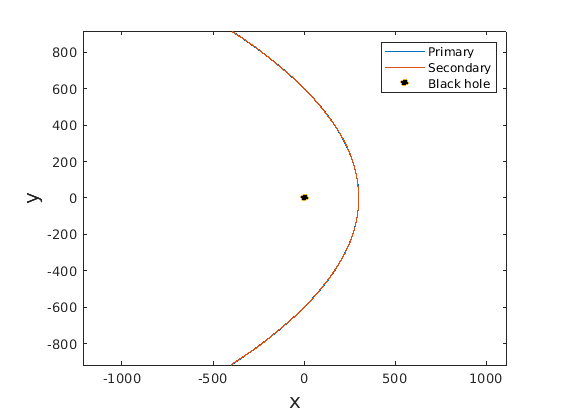
\includegraphics[width=\columnwidth]{../plots/3a_orbits_equalaxes.png}
					\caption{Orbits of two stars in a binary star system in the black hole rest frame.}
					\label{fig:3a}
				\end{subfigure}
				\hfill
				\begin{subfigure} {.5\columnwidth}
					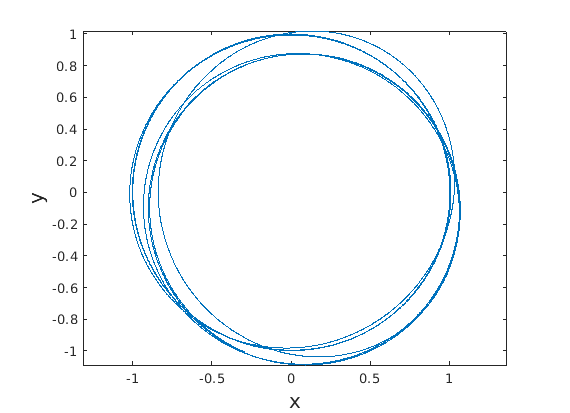
\includegraphics[width=\columnwidth]{../plots/3b_secondaryorbit.png}
					\caption{Orbit of secondary star in rest frame of primary star.}
					\label{fig:3b}
				\end{subfigure}\\
				
				\begin{subfigure} {\columnwidth}
					\centering
					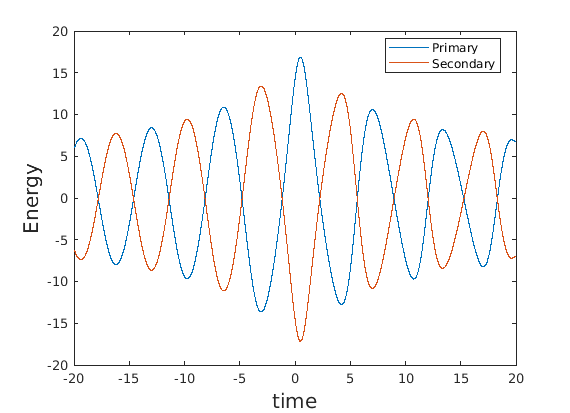
\includegraphics[width=.5\columnwidth]{../plots/3c_energy.png}
					\caption{Time evolution of dimensionless energies of the two stars in a binary star system.}
					\label{fig:3c}
				\end{subfigure}
				\caption{Plotted results for problems 3(a)--(c)}
				\label{fig:3.1}
			\end{figure}
			
			
			\begin{table}
				\centering
				\begin{tabular} {l l r r}
					\toprule
					\textbf{Quantity} & \textbf{Variable} & \textbf{D=3} & \textbf{D=0.1}\\
					\midrule
					\(t^{}_{0}\) & \texttt{t} & -19.9555 & -15.1290 \\
					\(x^{}_{p}\) & \texttt{x(1)}& -400.0000 & -980.0000 \\
					\(y^{}_{p}\) & \texttt{x(2)} & -916.7151 & -199.1975 \\
					\(v^{}_{px}\) & \texttt{x(3)} & 37.6166 & 44.6972 \\
					\(v^{}_{py}\) & \texttt{x(4)} & 24.4949 & 4.4721 \\
					\(x^{}_{s}\) & \texttt{x(5)} & -400.0000 & -980.0000 \\
					\(y^{}_{s}\) & \texttt{x(6)} & -915.7151 & -198.1975 \\
					\(v^{}_{sx}\) & \texttt{x(7)} & 36.6166 & 43.6972 \\
					\(v^{}_{sy}\) & \texttt{x(8)} & 24.4949 & 4.4721 \\
					\bottomrule
				\end{tabular}
				\caption{Summary of initial values of various physical quantities in the simulation and their variable names. These values are enlisted for values \(D=3\) and \(D=0.1\).}
				\label{table:3_dvalues}
			\end{table}
			
			
			
			
			
			\begin{enumerate} [label*=\textbf{(\alph*)}]
	
			% ---------------------------------- (a) ---------------------------------------------
	
				\item
					\subitem \textbf{Methods  --}
					The function \texttt{dxdy} defined in Matlab code file \emph{f.m} is modified to include black hole gravity terms in lines 7,8,11 and 12 of code \ref{code:3.f}. These modifications are done in accordance with the equations,
					\begin{equation}
						\begin{gathered}
							E_p = \frac{1}{2} m_p v_p^2 - \frac{G m_p M}{r_p} - \frac{G m_p m_s}{r_{ps}}, \\
							E_s = \frac{1}{2} m_s v_s^2 - \frac{G m_s M}{r_s} - \frac{G m_p m_s}{r_{ps}},
						\end{gathered}
					\end{equation}
					where, \(M\) is the mass of black hole and \(r_p\) and \(r_s\) are the distances from black hole to primary and secondary stars, respectively.
					
					\begin{figure} [h]
						\lstinputlisting[caption=f.m - Function defining values of velocities and accelerations of the two stars along the two axes., label=code:3.f]{../problem3d/f.m}
					\end{figure}
					
					In dimensionless units, the mass of black hole is given by,
					\begin{equation}
							\tilde{M} = \frac{M}{m_p+m_s} = \frac{M}{m}
							\label{eq:3-blackhole_mass}
					\end{equation}
					 In the given scenario, \(m_p = 3.2 M_\odot\), \(m_s = 0.8 M_\odot\) and \(M = 4 \times 10^6 M_\odot\). This gives us \(m = 3.2+0.8 = 4 M_\odot\). Consequently, using equations \ref{eq:dimensionless_mass_pos} and \ref{eq:3-blackhole_mass}, dimensionless masses are given by,
					 \begin{equation}
					 	\begin{gathered}
					 		\begin{aligned}
					 			\tilde{m}_p &= 0.8 \\
					 			\tilde{m}_s &= 0.2 \\
					 			\tilde{M} &= 10^6
					 		\end{aligned}
					 	\end{gathered}
				 		\label{eq:3-dimensionless_masses}
					 \end{equation}
					These values are assigned in the initial lines of the main code \emph{HVS.m} to variables \texttt{mp}, \texttt{ms} and \texttt{mb}, respectively.
					
					\begin{figure}
						\lstinputlisting[caption=initialc.m - Initial conditions for the simulation., label=code:3.initialc,
						firstline=5]{../problem3d/initialc.m}
					\end{figure}
					
					Next, the initial conditions are specified in the file \emph{initialc.m}, shown in code \ref{code:3.initialc}. The initial position of primary star with respect to black hole is given by,
					
					\begin{equation}
						x_p = X_{CM}^{} +r_p,
						\label{eq:3-primary_position}
					\end{equation}
					where, \(X_{CM}\) is the position of of centre of mass of binary from black hole, and \(r_p\) is the position of primary star with respect to centre of mass of binary. All these quantities are vectors and arrows have been dropped here (and later) for simplicity, and the approximation that centre of mass of the whole system lies within the black hole is assumed to be valid here, given that \(M \gg m_p,m_s\). 
					
					The value of \(X_{CM}^{}\) in equation \ref{eq:3-primary_position} is given by, 
					\begin{equation}
						X_{CM}^{} = (R \cos(f), R \sin(f)),
						\label{eq:3-xcm}
					\end{equation}
					where,
					\begin{equation}
						R = \frac{2 R_p}{1+ \cos(f)}.
						\label{eq:3-r}
					\end{equation}
					The angle \(f\), called \emph{true anomaly}, is the angle from point of closest approach and is a function of time. \(R_p\) is the \emph{periastron}, which is the distance of closest approach. The initial value of true anomaly is given as,
					\begin{equation}
						f_0 = - \cos^{-1} \left( \frac{D}{5} -1 \right),
						\label{eq:3-true_anomaly} 
					\end{equation}
					where, 
					\begin{equation}
						D = \frac{R_p}{R_t}
						\label{eq:3-d}
					\end{equation}
					
					For a given phase angle \(\phi\), the value of \(r_p\) in equation \ref{eq:3-primary_position} is given by,
					\begin{equation}
						r_p = (m_s \cos(\phi+\pi), m_s \sin (\phi+\pi))
						\label{eq:3-rp}
					\end{equation}
					
					Using equations \ref{eq:3-primary_position}, \ref{eq:3-xcm} and \ref{eq:3-rp}, we obtain the coordinates of primary star as,
					\begin{equation}
						\begin{gathered}
							x_{px} = R \cos(f) + m_s \cos(\phi+\pi) \\
							x_{py} = R \sin(f) + m_s \sin(\phi+\pi)
						\end{gathered}
						\label{eq:3-primary_positions_xy}
					\end{equation}
					
					Similarly, for secondary star,
					\begin{equation}
						x_s = X_{CM}^{} + r_s,
						\label{eq:3-secondary_position}
					\end{equation}
					\begin{equation}
						r_s = (m_p \cos(\phi), m_p \sin(\phi))
						\label{eq:3-rs}
					\end{equation}
					Using equations \ref{eq:3-xcm}, \ref{eq:3-secondary_position} and \ref{eq:3-rs}, we obtain the coordinates of secondary star as,
					\begin{equation}
						\begin{gathered}
							x_{sx} = R \cos(f) + m_p \cos(\phi) \\
							x_{sy} = R \sin(f) + m_p \sin(\phi).
						\end{gathered}
					\end{equation}
				
					For the given initial conditions,
					\begin{equation}
						R_0 = 10 R_t,
						\label{eq:3-r0_rt}
					\end{equation}
					where \(R_t\) is the \emph{tidal radius}, given by,
					\begin{equation}
						\nonumber R_t^{} = \left( \frac{M}{m} \right)^{\frac{1}{3}} a
					\end{equation}
					In dimensionless units, \textit{i.e.}, in units of \(a\), tidal radius is given by,
					\begin{equation}
						\tilde{R}_t = \left( \tilde{M} \right)^{\frac{1}{3}}.
						\label{eq:3-tidal_radius}
					\end{equation}
					Therefore, from equations \ref{eq:3-r0_rt} and \ref{eq:3-tidal_radius},
					\begin{equation}
						\tilde{R}_0 = 10 M^{\frac{1}{3}}	
						\label{eq:3-r0_m}
					\end{equation}
					
					Velocity of primary star is given by differentiating equation \ref{eq:3-primary_position} with respect to time as,
					\begin{equation}
						v_p = \dot{x}_p = \dot{X}_{CM}^{} +\dot{r}_p.
						\label{eq:3-vp}
					\end{equation}
					Time derivative of \(X_{CM}^{}\) is given by differentiating equation \ref{eq:3-xcm} as,
					\begin{equation}
						\begin{gathered}
							\begin{aligned}
								\dot{X}_{CM}^{} &= \frac{d}{dt} (R \cos(f)), \frac{d}{dt} (R \sin(f)) \\
								\Rightarrow \dot{X}_{CMx} &= \dot{R} \cos(f) - R \dot{f} \sin(f), \\
								\dot{X}_{CMy} &= \dot{R} \sin(f) + R \dot{f} \cos(f)
							\end{aligned}
						\end{gathered}
						\label{eq:3-vcm}
					\end{equation}
					Here, tilde has been dropped from dimensionless variables for simplicity and \(\dot{R}\) and \(\dot{f}\) are given as,
					\begin{equation}
						\dot{R} = \frac{M^{1/3}}{\sqrt{2D}} \sin(f),
						\label{eq:3-rdot}
					\end{equation}
					\begin{equation}
						\dot{f} = \frac{\sqrt{2}}{4} D^{-3/2} \left( 1+\cos(f) \right)^2 .
						\label{eq:3-fdot}
					\end{equation}
					
					The binary star system can be assumed to be in the similar initial conditions as the one considered in part \ref{Problem2} of this project, \textit{i.e.} a circular binary rotating counter-clockwise in x-y plane with stars initially located on x-axis (Changing the phase angle \(\phi\) updates this condition accordingly. For example, \(\phi = \pi/2\) moves the initial positions to lie on y-axis). This will give us the derivative of equation \ref{eq:3-rp}, \(\dot{r}_p\) as,
					\begin{equation}
						\begin{gathered}
							\begin{aligned}
								\dot{r}_{px} &= -m_s \sin(\phi + \pi), \\
								\dot{r}_{py} &= m_s \cos(\phi + \pi).
							\end{aligned}
						\end{gathered} 
						\label{eq:3-vp_binary}
					\end{equation}
					
					Similarly, equation \ref{eq:3-vp} for secondary star translates to,
					\begin{equation}
						v_s = \dot{x}_s = \dot{X}_{CM}^{} + \dot{r}_s
						\label{eq:3-vs}
					\end{equation}
					Value of \(X_{CM}^{}\) is given by equation set \ref{eq:3-xcm}, while the value of \(r_s\) can be computed for secondary star using the method similar to the one used for primary star for equation set \ref{eq:3-vp_binary}, adopted from part \ref{Problem2} of the project. Using equation \ref{eq:3-rs} this gives us,
					\begin{equation}
						\begin{gathered}
							\begin{aligned}
								\dot{r}_{sx} &= -m_p \sin(\phi), \\
								\dot{r}_{sy} &= m_p \cos(\phi).
							\end{aligned}
						\end{gathered} 
						\label{eq:3-vs_binary}
					\end{equation}
				
					At \(t=0\), the binary passes through the periastron. This implies that the evolution of code needs to begin at time \(t<0\), which can be obtained as a function of initial true anomaly \(f_0\) discussed in equation \ref{eq:3-true_anomaly}. This gives us the initial time of 
					\begin{equation}
						t_0 = \frac{\sqrt{2}}{3} D^{3/2} \tan \left( \frac{f_0}{2} \right) \left( 3+ \tan^2 \left( \frac{f_0}{2} \right) \right) 
						\label{eq:3-initial_time}
					\end{equation}
				
					This gives us a complete set of initial conditions that can be used for simulation -- initial time, initial positions and initial velocities. These relations can be used in the Matlab file \emph{initialc.m} given in code \ref{code:3.initialc}, to define the initial conditions. \\
\newpage					
					To summarize,
					\begin{itemize}
						\item The dimensionless values of masses (equation set \ref{eq:3-dimensionless_masses}) and \(D=3\) (equation \ref{eq:3-d}) are initialized in the beginning of file \emph{HVS.m}.
						\item In file \emph{initialc.m}, shown in code \ref{code:3.initialc}, values of tidal radius, \(R_t\) (equation \ref{eq:3-tidal_radius}) and initial distance between binary and black hole, \(R_0\) (equation \ref{eq:3-r0_rt}) are defined in lines 1 and 2.
						\item The values of \(\dot{X}_{CM}^{}\) (velocity equation set \ref{eq:3-vcm}) along the two axes are defined in lines 8 and 9.
						\item Calculating the values of \(\dot{X}_{CM}^{}\) requires values of true anomaly (\(f_0\)), time derivative of radial distance \(\dot{R}\) and time derivative of true anomaly \(\dot{f}\), given by equations \ref{eq:3-true_anomaly}, \ref{eq:3-rdot} and \ref{eq:3-fdot}, respectively. These values are defined in lines 3--6.
						\item A phase angle \(\phi = \pi/2\) is assumes and initialized in line 11.
						\item Initial time \(t_0\) is calculated using equation \ref{eq:3-initial_time} in line 17--18.
						\item Initial positions of the two stars are computed in lines 19--20 and 23--24 using equation sets \ref{eq:3-rp} and \ref{eq:3-rs}.
						\item The values of initial velocities derived in equations \ref{eq:3-vp} and \ref{eq:3-vs} as assigned in lines 21--22 and 25--26.
						\item Values of velocities depend on velocity of centre of mass as well as velocity of each star in the binary. Velocity of centre of mass is already defined in lines 8--9, as mentioned above, while the velocities of each star along the two axes are defined in lines 12--15 using equation sets \ref{eq:3-vp_binary} and \ref{eq:3-vs_binary}.
					\end{itemize}
					
					\begin{figure} [h]
						\lstinputlisting[caption=script4.m - Code snippet to plot the trajectories of stars in black hole rest frame., label=code:3.script4a,
										firstline=12, firstnumber=12,
										lastline=20] {../problem3d/script4.m}
					\end{figure}
					
					Using the above methods, the initial conditions are defined. Upon executing the code \emph{HVS.m}, a file named \emph{out} is created. The plotting of trajectories in black hole rest frame is done using Matlab code \emph{script4.m}, a snippet of which is shown in code \ref{code:3.script4a}.
					
					\subitem \textbf{Results  --}
					The plot of obtained trajectories of the binary stars in the black hole rest frame is shown in figure \ref{fig:3a}. The numerically computed values of initial conditions are summarised in table \ref{table:3_dvalues}.
					
					\subitem \textbf{Discussions  --}
					The trajectory of the centre of mass of binary appears to be parabolic. This can be confirmed if the energy of the binary turns out to be zero. Also, though the plot seems to show a single line of trajectory, on zooming in, the individual tracks of the two stars can be resolved. The structure and separation of binary does not seem to be affected by the interaction on close approach of the system at periastron.
	
			% ---------------------------------- (b) ---------------------------------------------

				\item
					\begin{figure} [h]
						\lstinputlisting[caption=script4.m - Code snippet to plot the trajectory of secondary star in the rest frame of primary mass., label=code:3.script4b,
						firstline=22, firstnumber=22,
						lastline=25] {../problem3d/script4.m}
					\end{figure}
				
					\subitem \textbf{Methods  --} Using the output file \emph{out}, the trajectory of secondary star in units of dimensionless position in the comoving frame of primary star is plotted using the code snippet shown in code \ref{code:3.script4b}.
					
					\subitem \textbf{Results  --}
					The plot obtained is shown in figure \ref{fig:3b}.
					
%					\subitem \textbf{Discussions  --}
	
			% ---------------------------------- (c) ---------------------------------------------
	
				\item
					\begin{figure} [h]
						\lstinputlisting[caption=script4.m - Code snippet to plot evolution of energies of binary stars over time, label=code:3.script4c,
						firstline=27, firstnumber=27,
						lastline=32] {../problem3d/script4.m}
					\end{figure}
				
					\subitem \textbf{Methods  --}
					The energies of primary and secondary stars is given by,
					\begin{equation}
						\begin{gathered}
							E_p = \frac{1}{2} m_p v_p^2 - \frac{G m_p M}{r_p} - \frac{G m_p m_s}{r_{ps}} \\
							E_s = \frac{1}{2} m_s v_s^2 - \frac{G m_s M}{r_s} - \frac{G m_p m_s}{r_{ps}}
						\end{gathered}
					\label{eq:3-energies}
					\end{equation}
					The energies in dimensionless units computed using \emph{HVS.m} and \emph{energy.m} are imported from \emph{out} file and plotted using the code snippet shown in code \ref{code:3.script4c}. 
					
					\subitem \textbf{Results  --}
					The plot of evolution of energies of primary and secondary stars is shown in figure \ref{fig:3c}.
					
					\subitem \textbf{Discussions  --}
					The total dimensionless energy of the system remains constant and equal to zero over time, as can be observed from figure \ref{fig:3c}.
	
			% ---------------------------------- (d) ---------------------------------------------
	
				\item
					\subitem \textbf{Methods  --}
					Using all the same programs used in parts (a)--(c), the value of \(D\) is updated to a new value of \(0.1\) in Matlab code \emph{HVS.m}. The plotting of data generated in \emph{out} file is also done using the same codes. 
					
					\begin{figure} [h]
						\begin{subfigure} {.5\columnwidth}
							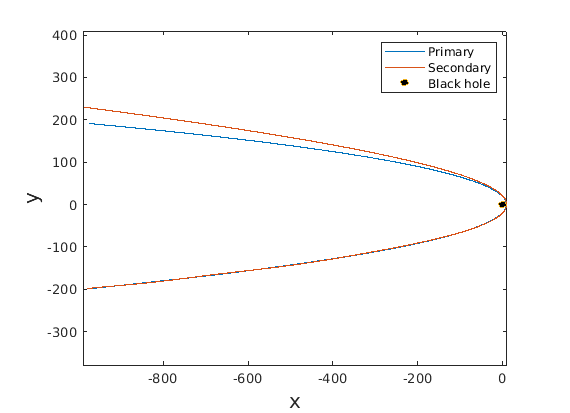
\includegraphics[width=\columnwidth]{../plots/3d_orbitsdisruption_equalaxes.png}
							\caption{Orbits of two stars in a binary star system in the black hole rest frame. Note that the binary separation increases over time after tidal interaction with black hole.}
							\label{fig:3da}
						\end{subfigure}
						\hfill
						\begin{subfigure} {.5\columnwidth}
							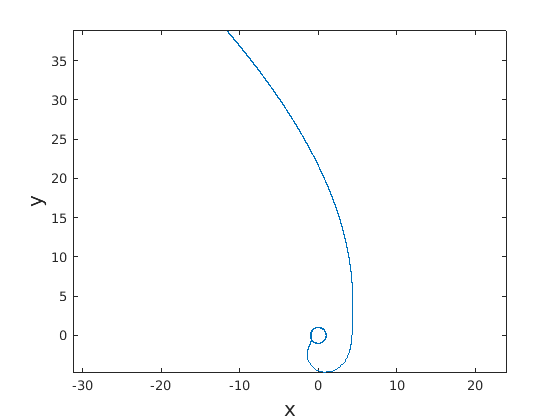
\includegraphics[width=\columnwidth]{../plots/3d_secondaryorbitdisruption_equalaxes.png}
							\caption{Orbit of secondary star in rest frame of primary star. The stars are seen to depart away from each other at later times}
							\label{fig:3db}
						\end{subfigure}\\
						
						\begin{subfigure} {\columnwidth}
							\centering
							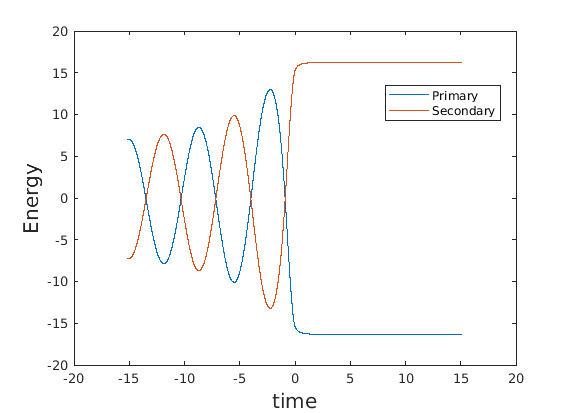
\includegraphics[width=.5\columnwidth]{../plots/3d_energy.png}
							\caption{Time evolution of dimensionless energies of the two stars in a binary star system. The plot changes abruptly at \(t=0\), \textit{i.e.} after tidal interaction.}
							\label{fig:3dc}
						\end{subfigure}
						\caption{Plotted results for problem 3(d).}
						\label{fig:3.2}
					\end{figure}
					
					\subitem \textbf{Results  --} 
					The plots generated are shown in figure \ref{fig:3.2}. The trajectory in terms of dimensionless position of the two stars in black hole rest frame is shown in figure \ref{fig:3da}. The orbit of the secondary star in rest frame of primary star is shown in figure \ref{fig:3db}. The evolution of dimensionless energies of the two stars over time is shown in figure \ref{fig:3dc}. The values of initial parameters computed in the code are enlisted in table \ref{table:3_dvalues}.
					
					\subitem \textbf{Discussions  --}
					The trajectory of the centre of mass of binary still appears to be parabolic. The separation of the binary is affected in later times, after the tidal interaction with the black hole. The binary separates over time as seen in the upper left corner of figure \ref{fig:3da}. This break up of binary is essentially an effect of tidal interaction of binary with the black hole. Evidently, this becomes prominent as the binary passes very close to the super massive black hole, such as the one found in the centre of our galaxy.
					
					The star detaches from binary after the tidal interaction. This is seen in figure \ref{fig:3db}. In the rest frame of primary star, the secondary star is seen to initially encircle as the binary rotates, evident in lower central circular region of figure \ref{fig:3db}. After gravitational interaction,the secondary star begins to increasingly move away from primary star.
					
					The total energy of the binary, which is the sum of the energies of the two stars is conserved over time and is zero. After time \(t=0\), when the binary reaches the periastron, the energy of primary star becomes extremely negative, while the energy of the secondary star becomes extremely positive. This indicates that orbit of primary star become more bound to the black hole and vice versa. This suggests more strongly that deviations in orbits of stars of the binary are essentially due to gravitational interactions between binary and black hole, in case the point of approach is closer than some limiting value, decided by the value of \(D\). 
					
				\item
					\subitem \textbf{Methods --}
					From previous part, we know that the star ejected from the binary after tidal interaction is the secondary star. From equation \ref{eq:3-energies}, we can estimate the final velocity at \(r=\infty\) using the value of velocity obtained from our numerical results in \emph{out} file. At such large distances the following two approximations can be made safely,
					\begin{equation}
						\begin{gathered}
							\frac{G m_s M}{r_s} \approx 0, \\
							\frac{G m_p m_s}{r_{ps}} \approx 0 .
						\end{gathered}
					\end{equation}
					This gives us,
					\begin{equation}
						\begin{gathered}
							\begin{aligned}
								E_s &\approx \frac{1}{2} m_s v_s^2 \\
								\Rightarrow v_s &\approx \sqrt{\frac{2 E_s}{m_s}}
							\end{aligned}
						\end{gathered}
						\label{eq:3-secondary_velocity_infty}
					\end{equation}
				
					\subitem \textbf{Results --}
					Numerical values obtained from the simulation give an eventual dimensionless energy of \(\tilde{E}_s \approx 16.2244\) for the secondary star. Substituting non-dimensionless values in equation \ref{eq:3-secondary_velocity_infty}, we get,
					\begin{equation}
						\begin{gathered}
							\begin{aligned}
								v_s &= \sqrt{\frac{2 \tilde{E}_s G m^2}{m_s a}} \\
								&= \sqrt{\frac{2 \times 16.2244 \times (6.67\times 10^{-11}) \times (4M_\odot)^2_{}}{(7\times R_\odot)\times(0.8 \times M_\odot)}} \\
								&= \sqrt{\frac{618.38 \times 10^{-11} M_\odot}{R_\odot}} \\
								&\approx 4204 \text{ km/s}.
							\end{aligned}
						\end{gathered}
						\label{eq:3-velocity_at_inf}
					\end{equation}
					Thus, for the secondary star, detached from the binary, we obtain a velocity of approximately 4204 km/s at a distance \(r=\infty\). 
					
				\item
				
				\begin{figure} [h]
					\lstinputlisting[caption=HVS.m - Program to perform simulation for different values of \(D\),label=code:3f.hvs , 
									firstline=5, firstnumber=5] {../problem3f/HVS.m}
				\end{figure}
				
				\begin{figure} [h]
					\begin{subfigure} {.45\linewidth}
						\lstinputlisting[caption=initialc.m - Initial velocities for clockwise rotating binaries., label=code:3f.initialc_retrograde , 
										firstline=16, firstnumber=16,
										lastline=19] {../problem3f/initialc_retrograde.m}
					\end{subfigure} %
					\hfill
					\begin{subfigure} {.45\linewidth}
						\lstinputlisting[caption=initialc.m - Initial velocities for counter-clockwise rotating binaries., label=code:3f.initialc_prograde , 
										firstline=16, firstnumber=16,
										lastline=19] {../problem3f/initialc_prograde.m}
					\end{subfigure}
				\end{figure}
			
				\begin{figure} [h]
					\lstinputlisting[caption=script4.m - Program to collectively plot orbital trajectories for multiple data files in a directory. The commented lines 29--34 can be used to plot binary energy evolution instead., label=code:3f.script4 ,
									lastline=43] {../problem3f/script4.m}
				\end{figure}
				
				\subitem \textbf{Methods --}
				To answer whether the orientation of binary rotation affects the outcomes of our simulation, the orbital trajectories and energies of clockwise and counter-clockwise rotating binaries are probed. These simulations are performed for values of \(D =\) 1.0, 0.5, 0.1, 0.025, 0.0125 and 0.01. Code \ref{code:3f.hvs} shows the program to perform simulation similar to one performed in previous section for different values of \(D\) iteratively.
				
				The initial conditions for clockwise and counter-clockwise rotating binaries differ in their directions of initial velocities. Codes \ref{code:3f.initialc_retrograde} and \ref{code:3f.initialc_prograde} can be compared to mark the differences in initial velocities of the two types of binaries. Rest of the code is similar to code \ref{code:3.initialc}.
				
				Once a collection of output data files for different values of \(D\) for each type of binary is obtained, codes \ref{code:3.script4a} and \ref{code:3.script4c} can be used to plot orbits and energy evolution for each file. A slightly efficient program to plot and save multiple figures at once is given in code \ref{code:3f.script4}.
				
				\begin{figure} [h]
					\centering
					\begin{subfigure} {.425\linewidth}
						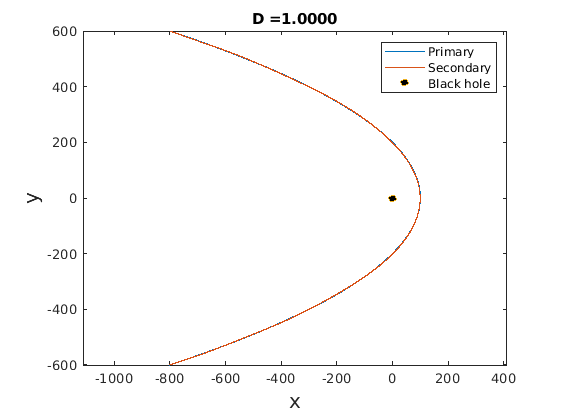
\includegraphics[width=\linewidth, height =.55\linewidth] {../plots/3f/retrograde_orbits/6.png}\\
						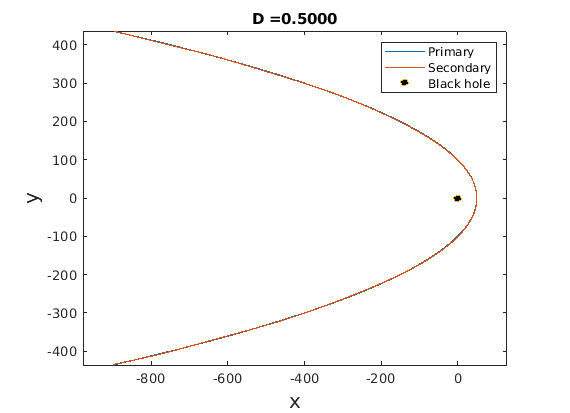
\includegraphics[width=\linewidth, height =.55\linewidth] {../plots/3f/retrograde_orbits/5.png}\\
						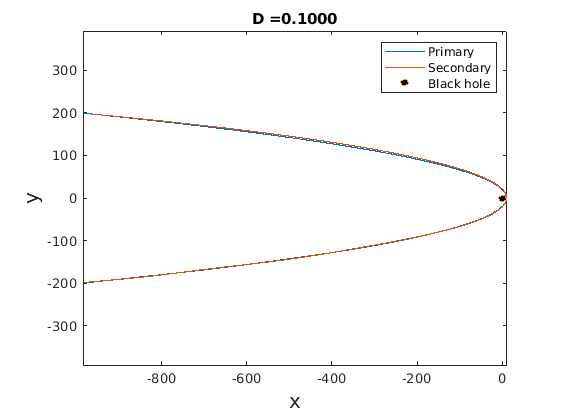
\includegraphics[width=\linewidth, height =.55\linewidth] {../plots/3f/retrograde_orbits/4.png}\\
						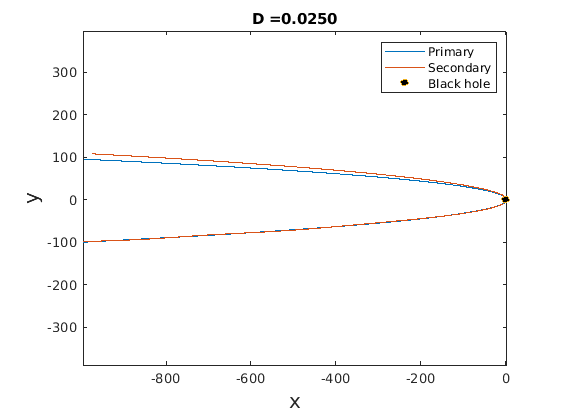
\includegraphics[width=\linewidth, height =.55\linewidth] {../plots/3f/retrograde_orbits/3.png}\\
						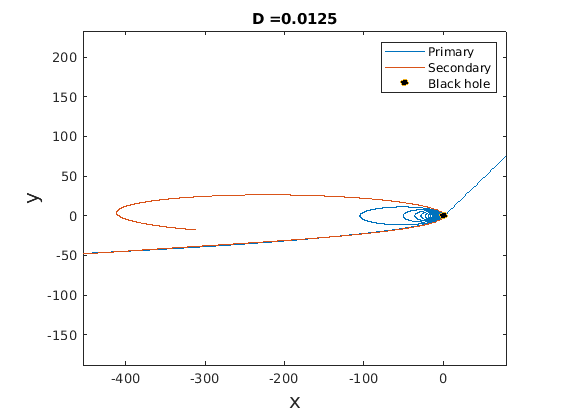
\includegraphics[width=\linewidth, height =.55\linewidth] {../plots/3f/retrograde_orbits/2.png}\\
						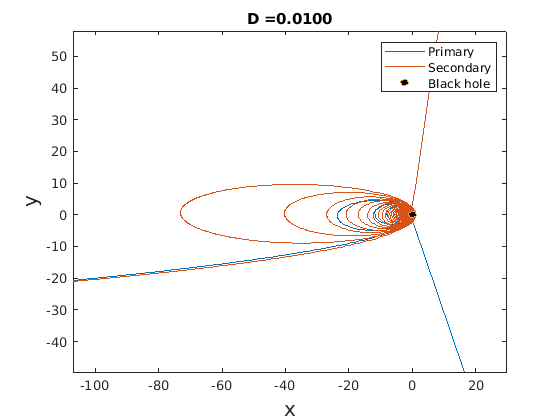
\includegraphics[width=\linewidth, height =.55\linewidth] {../plots/3f/retrograde_orbits/1.png}
					\end{subfigure} %
					\hspace{1cm}
					\begin{subfigure} {.425\linewidth}
						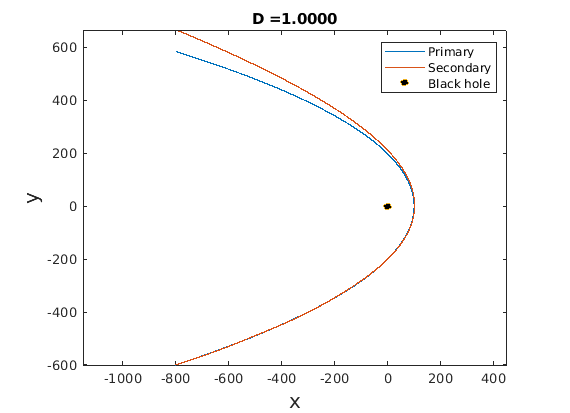
\includegraphics[width=\linewidth, height =.55\linewidth] {../plots/3f/prograde_orbits/6.png}\\
						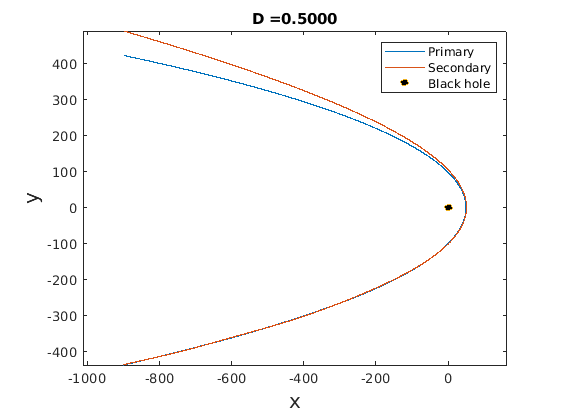
\includegraphics[width=\linewidth, height =.55\linewidth] {../plots/3f/prograde_orbits/5.png}\\
						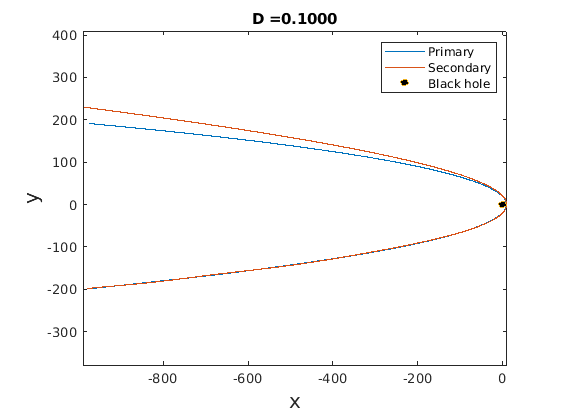
\includegraphics[width=\linewidth, height =.55\linewidth] {../plots/3f/prograde_orbits/4.png}\\
						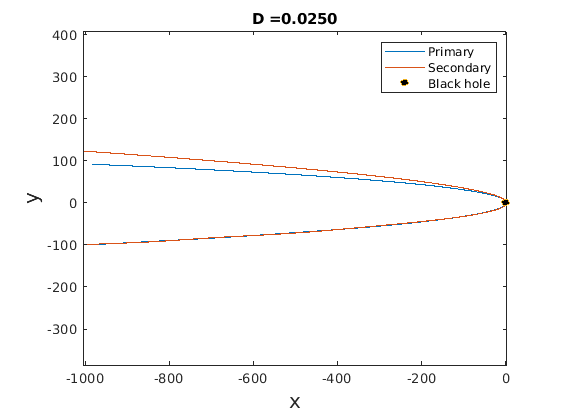
\includegraphics[width=\linewidth, height =.55\linewidth] {../plots/3f/prograde_orbits/3.png}\\
						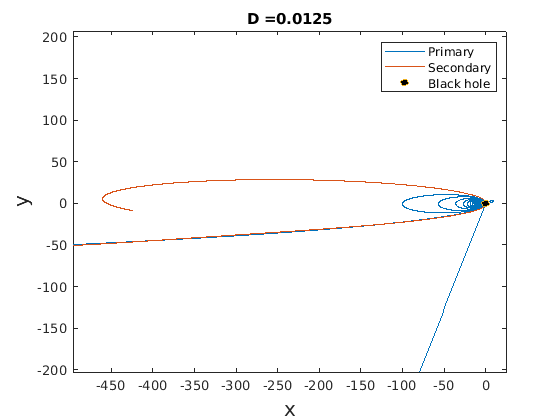
\includegraphics[width=\linewidth, height =.55\linewidth] {../plots/3f/prograde_orbits/2.png}\\
						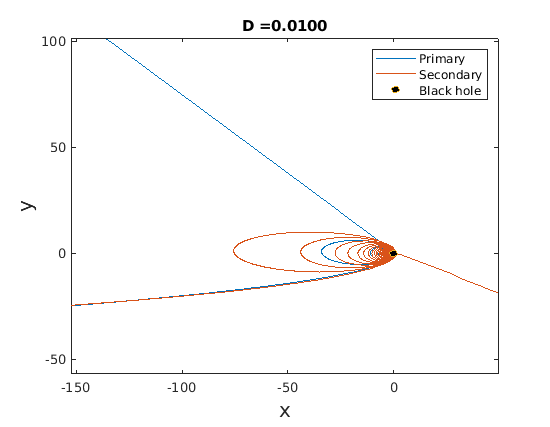
\includegraphics[width=\linewidth, height =.55\linewidth] {../plots/3f/prograde_orbits/1.png}
					\end{subfigure}
					\caption{A comparison of trajectories of clockwise (left) and counter-clockwise (right) binaries for different values of penetration factor \(D\) = 1.0, 0.5, 0.1, 0.025, 0.0125 and 0.01, for the cases of tidal breakups of binaries. Some plots are zoomed in for better visualization.}
					\label{fig:3f-orbits_pro_retro}
				\end{figure}
			
				\begin{figure} [h]
					\centering
					\begin{subfigure} {.425\linewidth}
						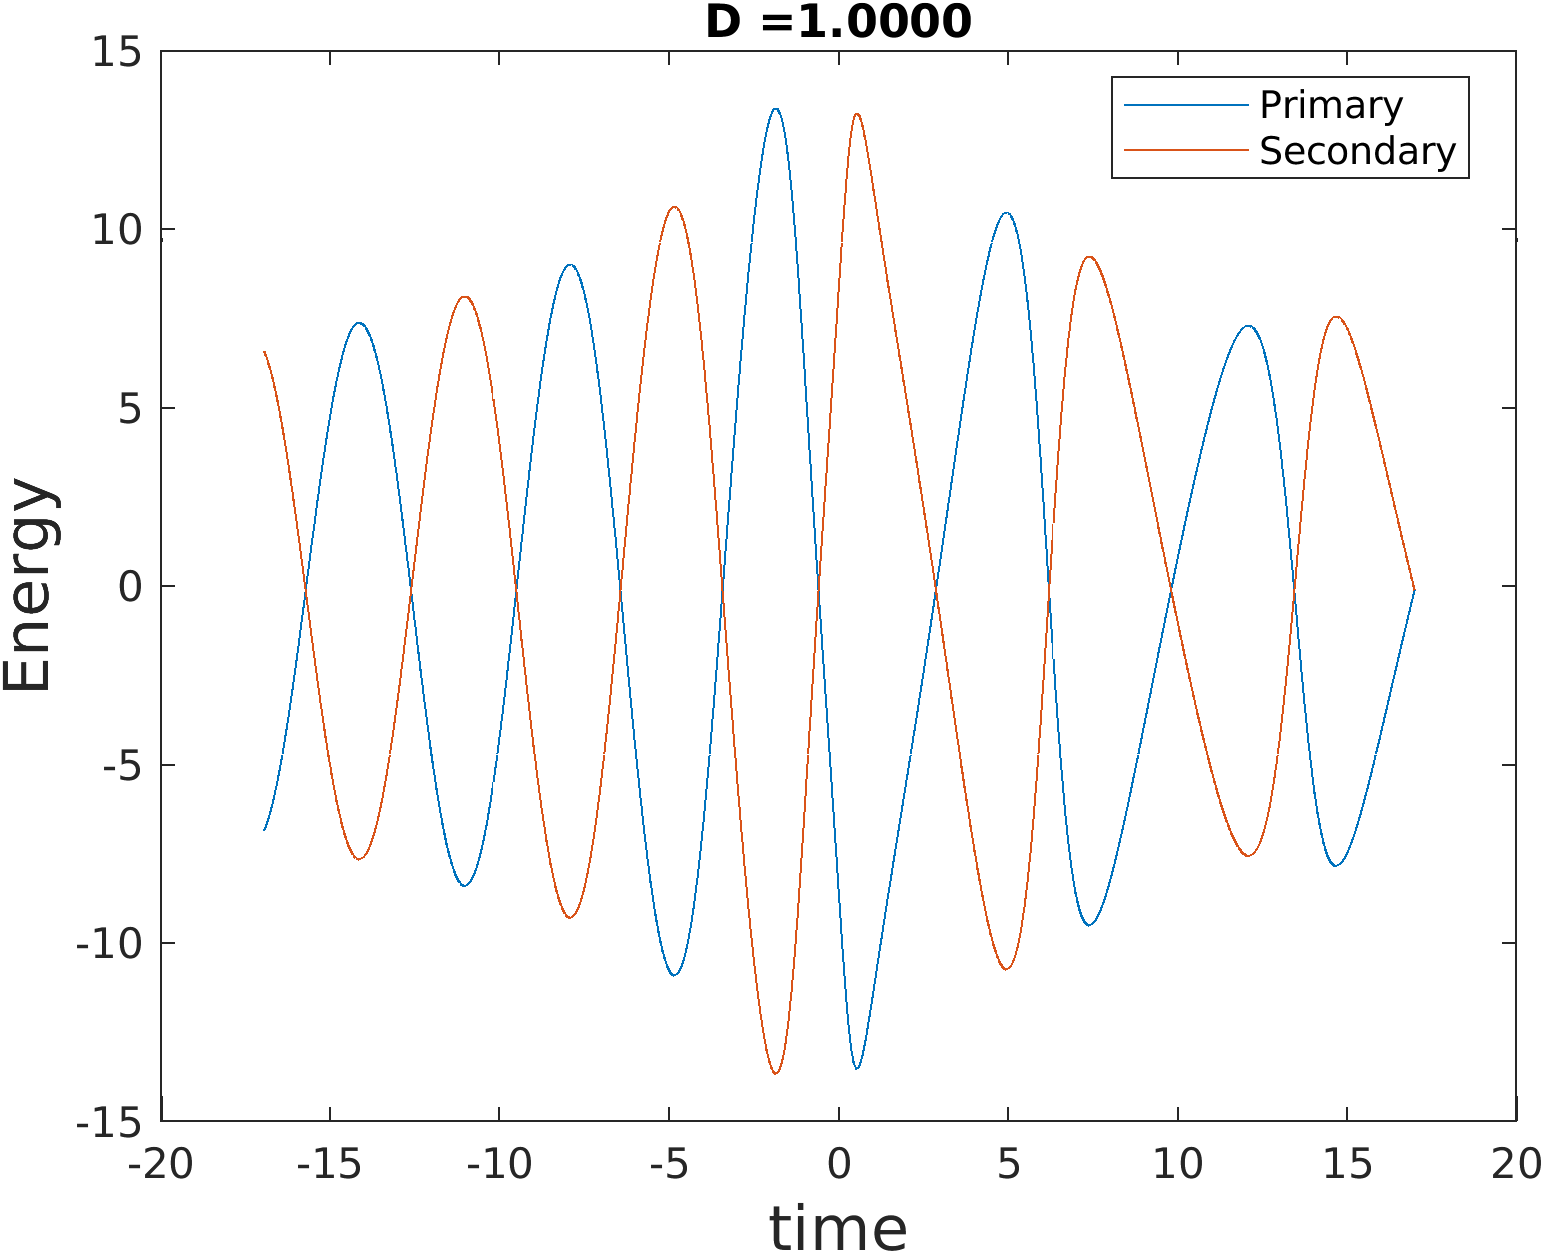
\includegraphics[width=\linewidth, height =.55\linewidth] {../plots/3f/retrograde_energies/6.png}\\
						\vspace{1.5mm}
						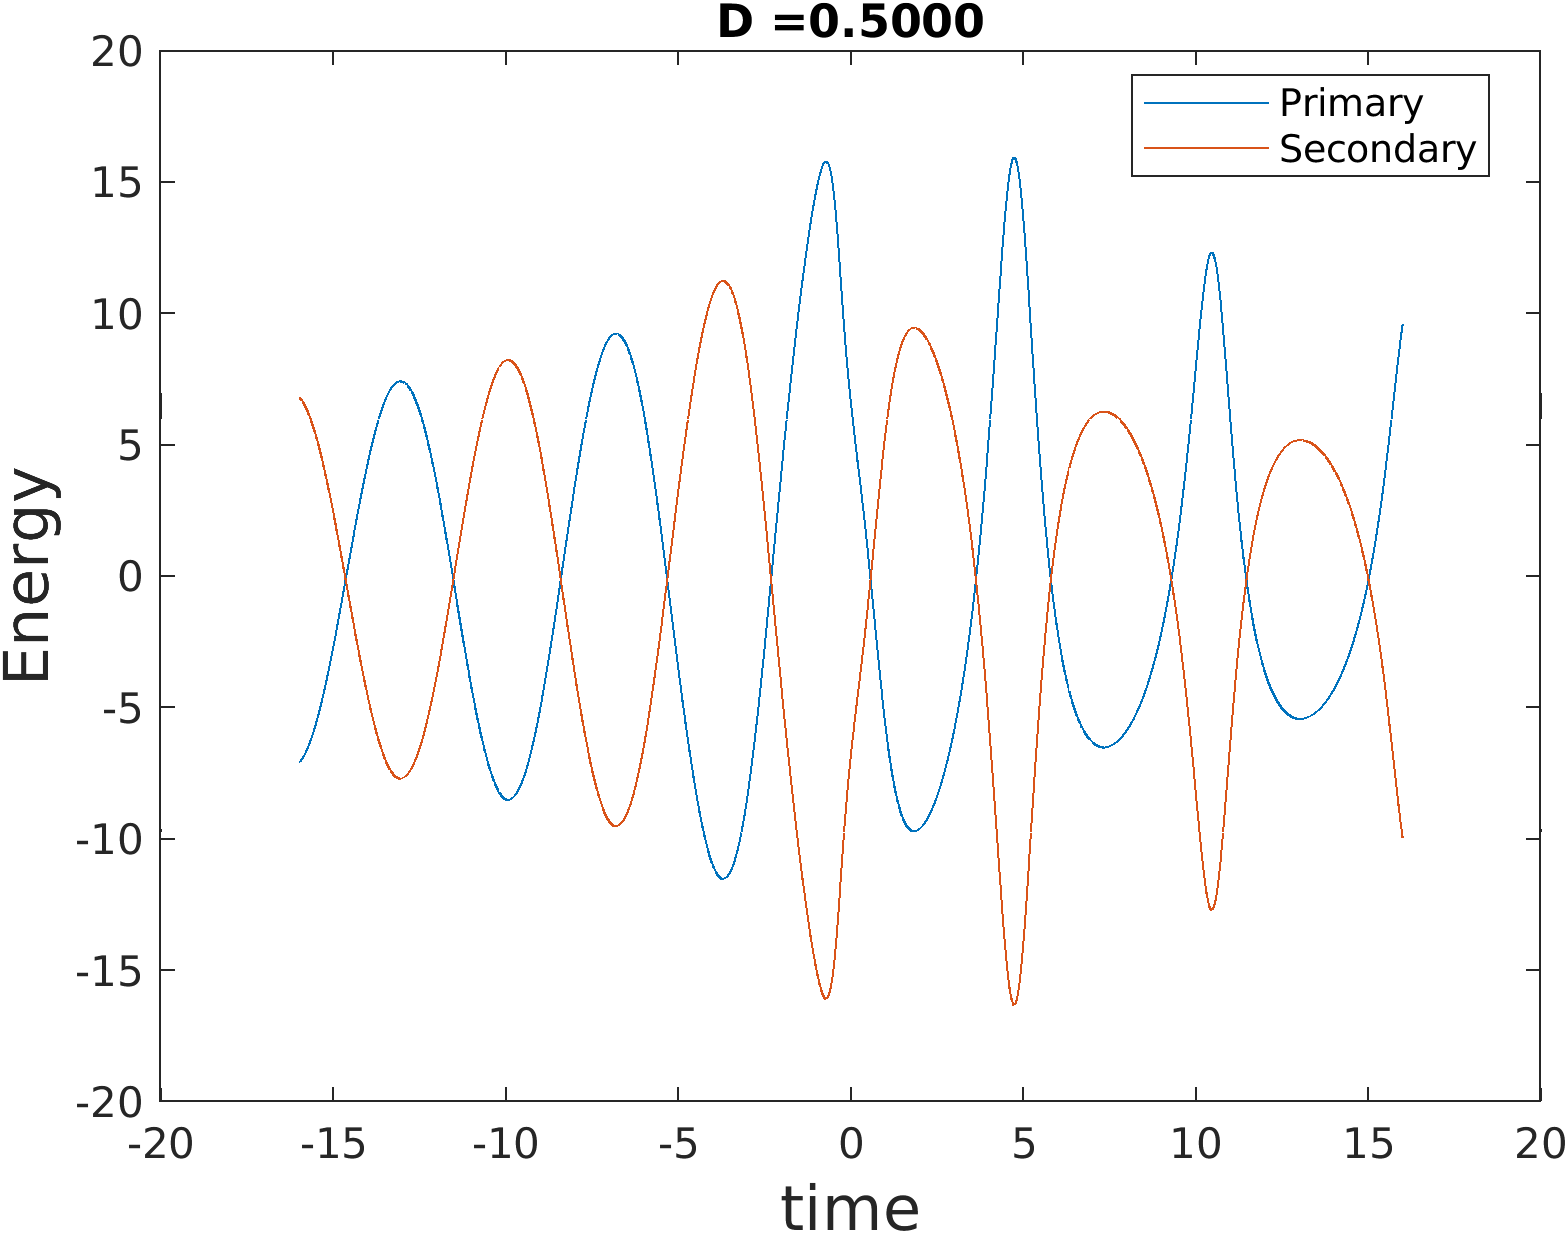
\includegraphics[width=\linewidth, height =.55\linewidth] {../plots/3f/retrograde_energies/5.png}\\
						\vspace{1.5mm}
						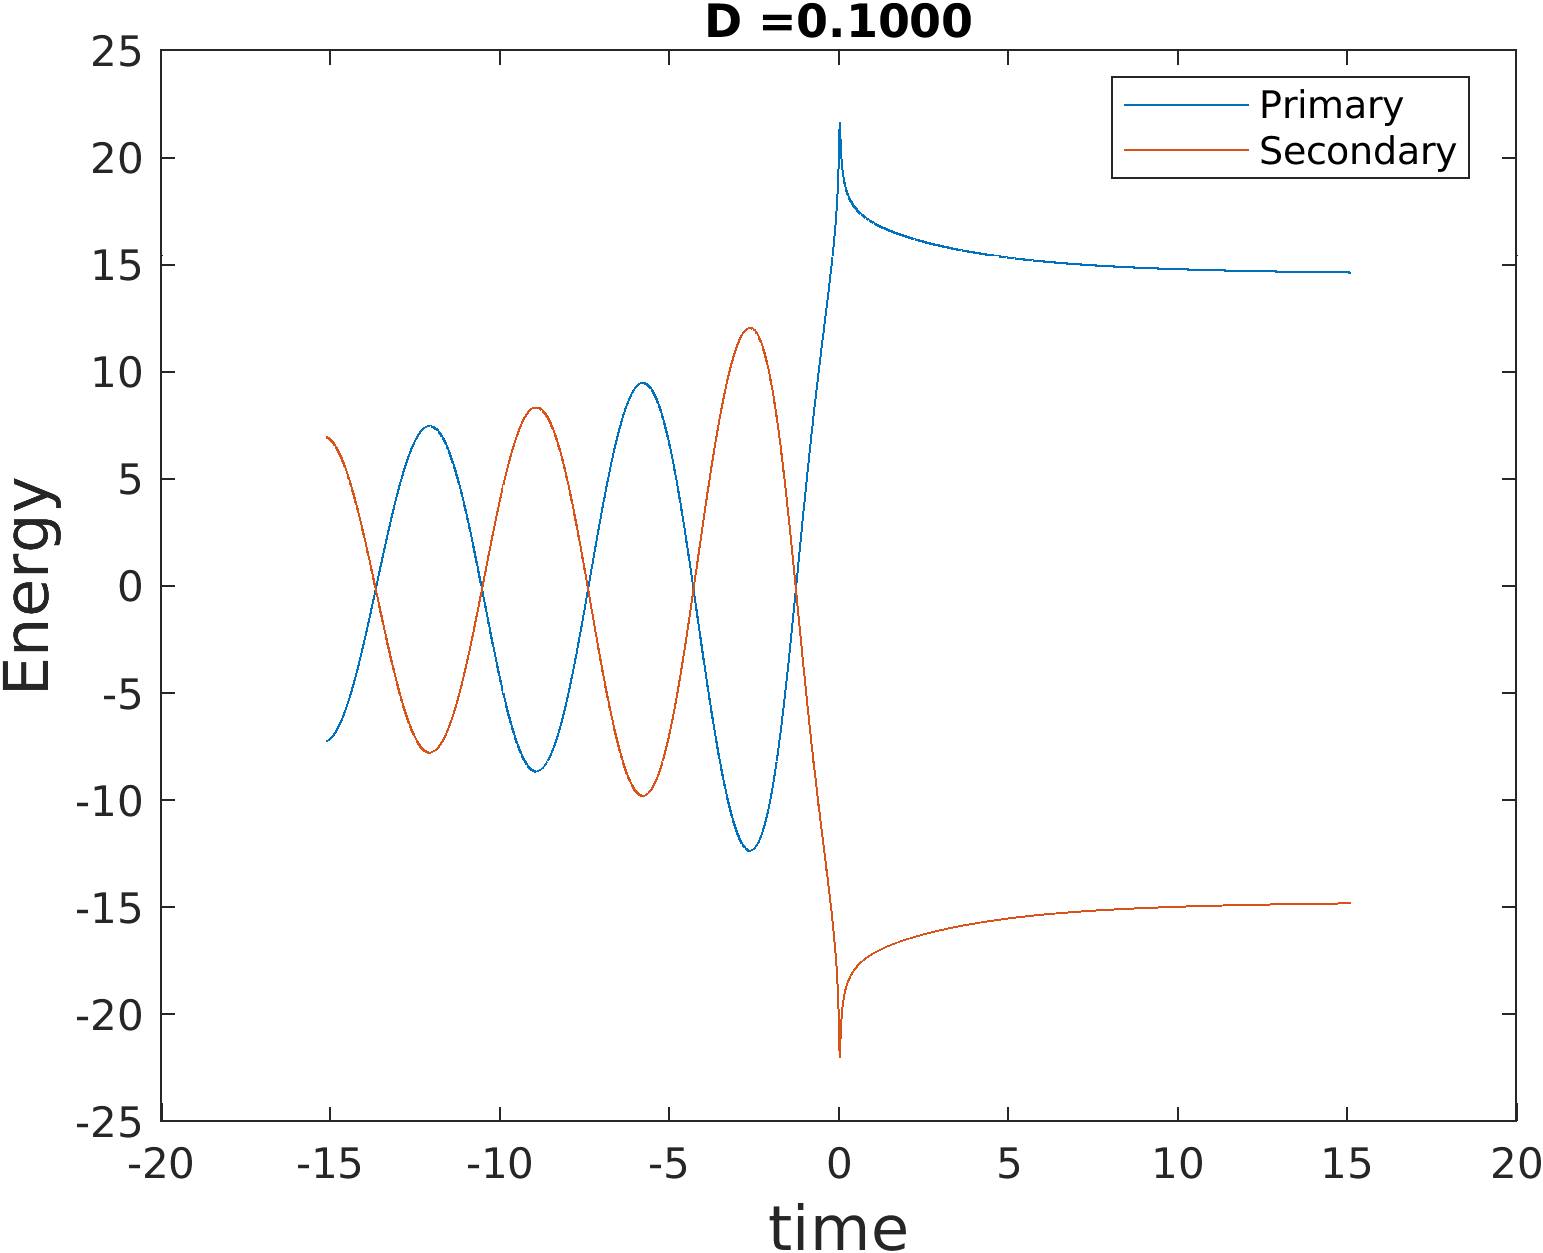
\includegraphics[width=\linewidth, height =.55\linewidth] {../plots/3f/retrograde_energies/4.png}\\
						\vspace{1.5mm}
						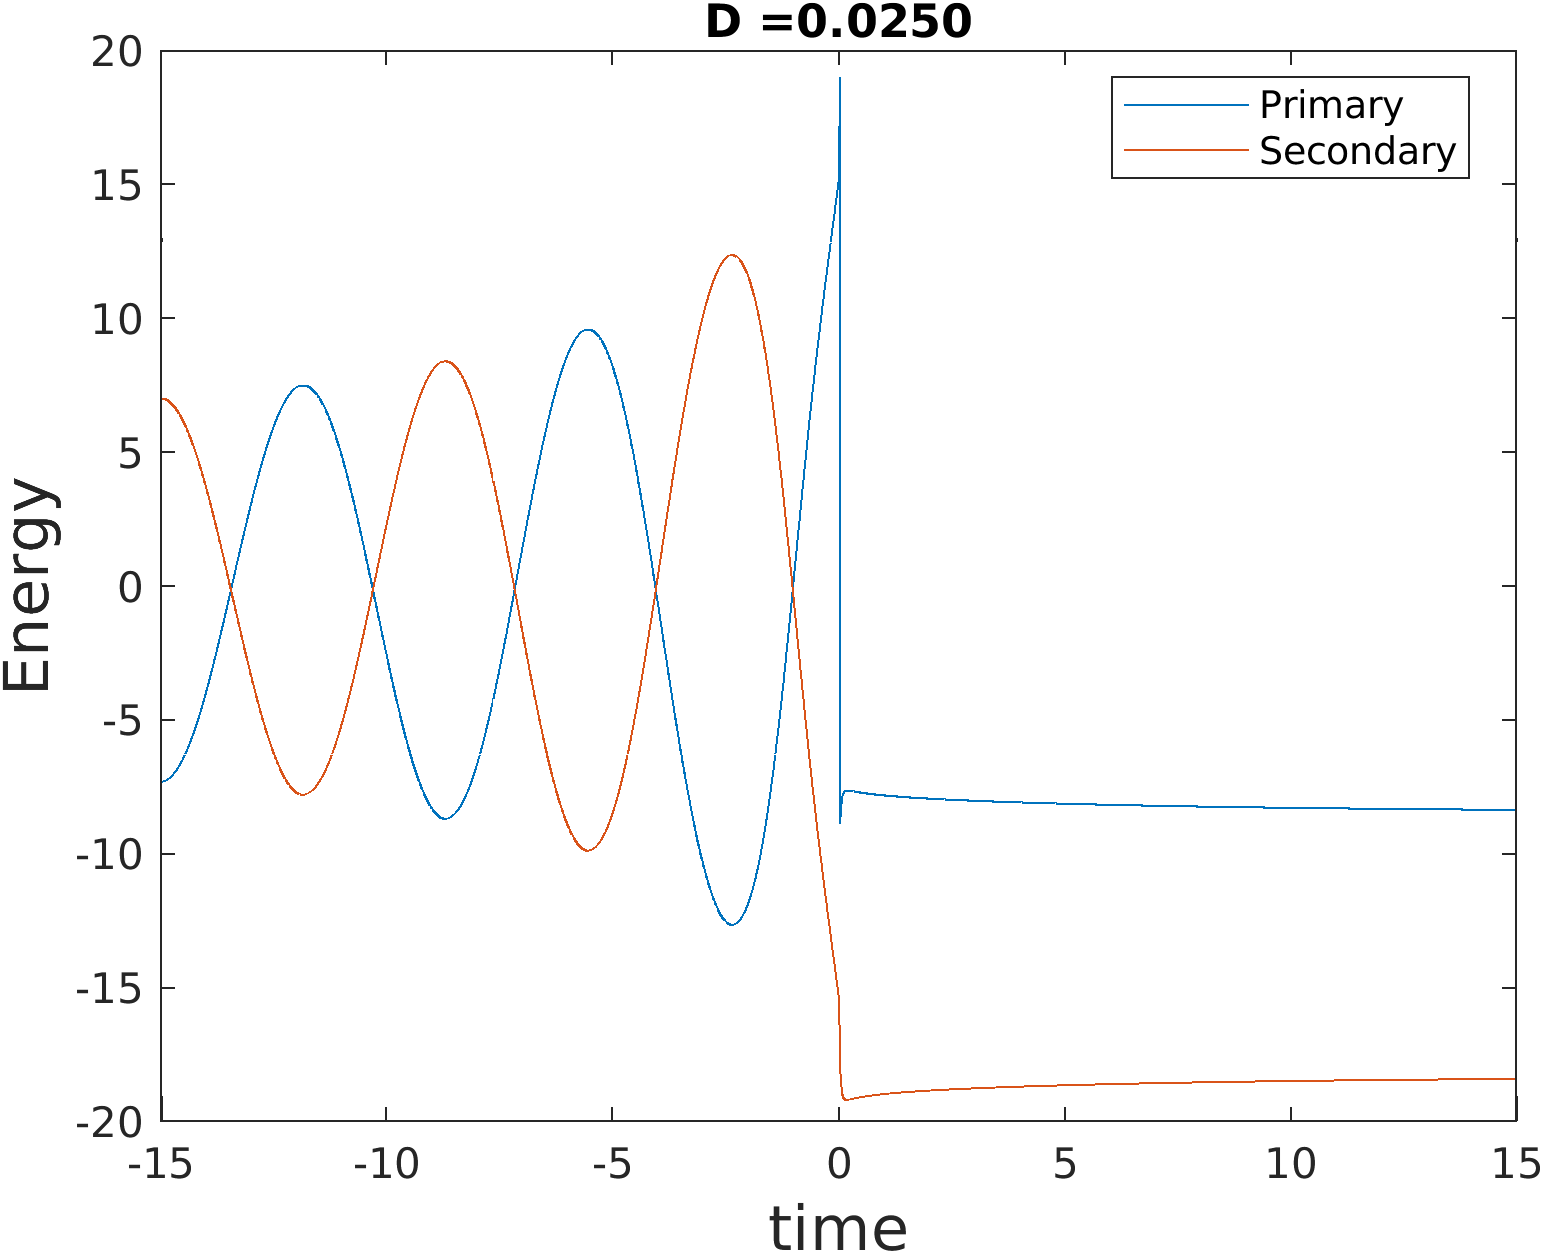
\includegraphics[width=\linewidth, height =.55\linewidth] {../plots/3f/retrograde_energies/3.png}\\
						\vspace{1.5mm}
						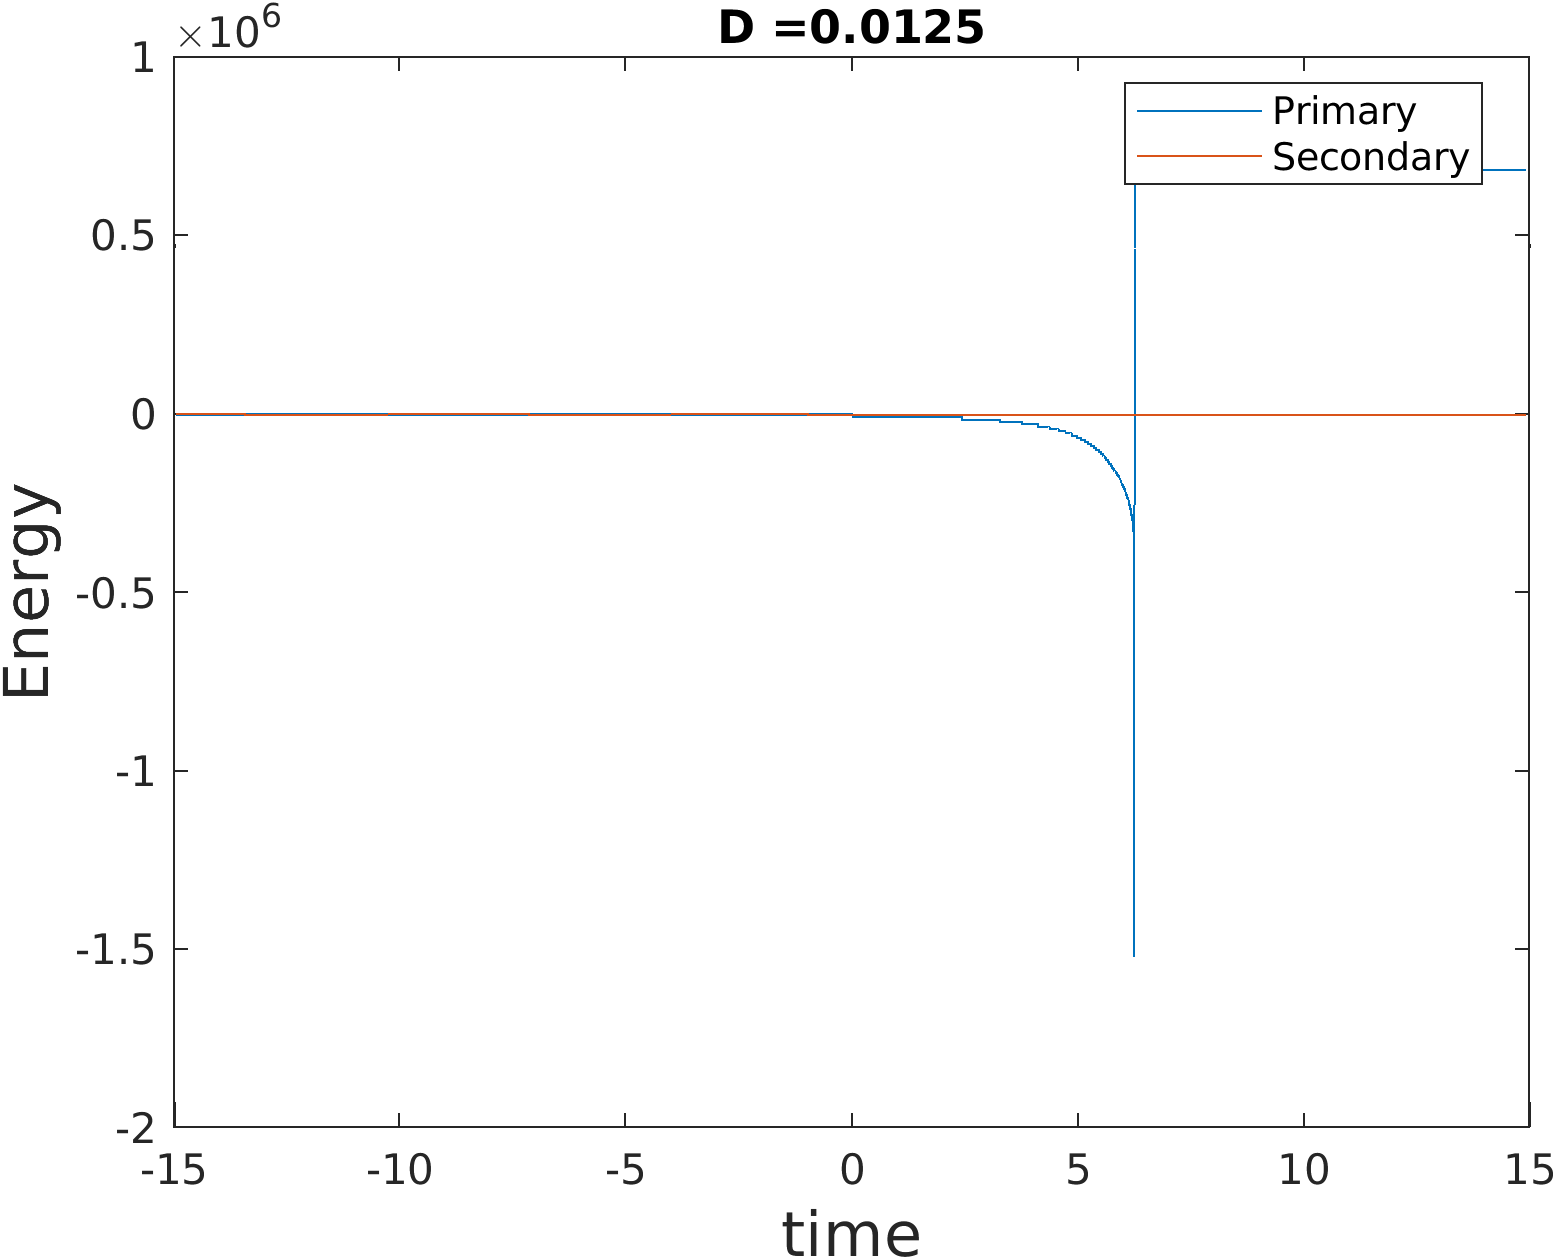
\includegraphics[width=\linewidth, height =.55\linewidth] {../plots/3f/retrograde_energies/2.png}\\
						\vspace{1.5mm}
						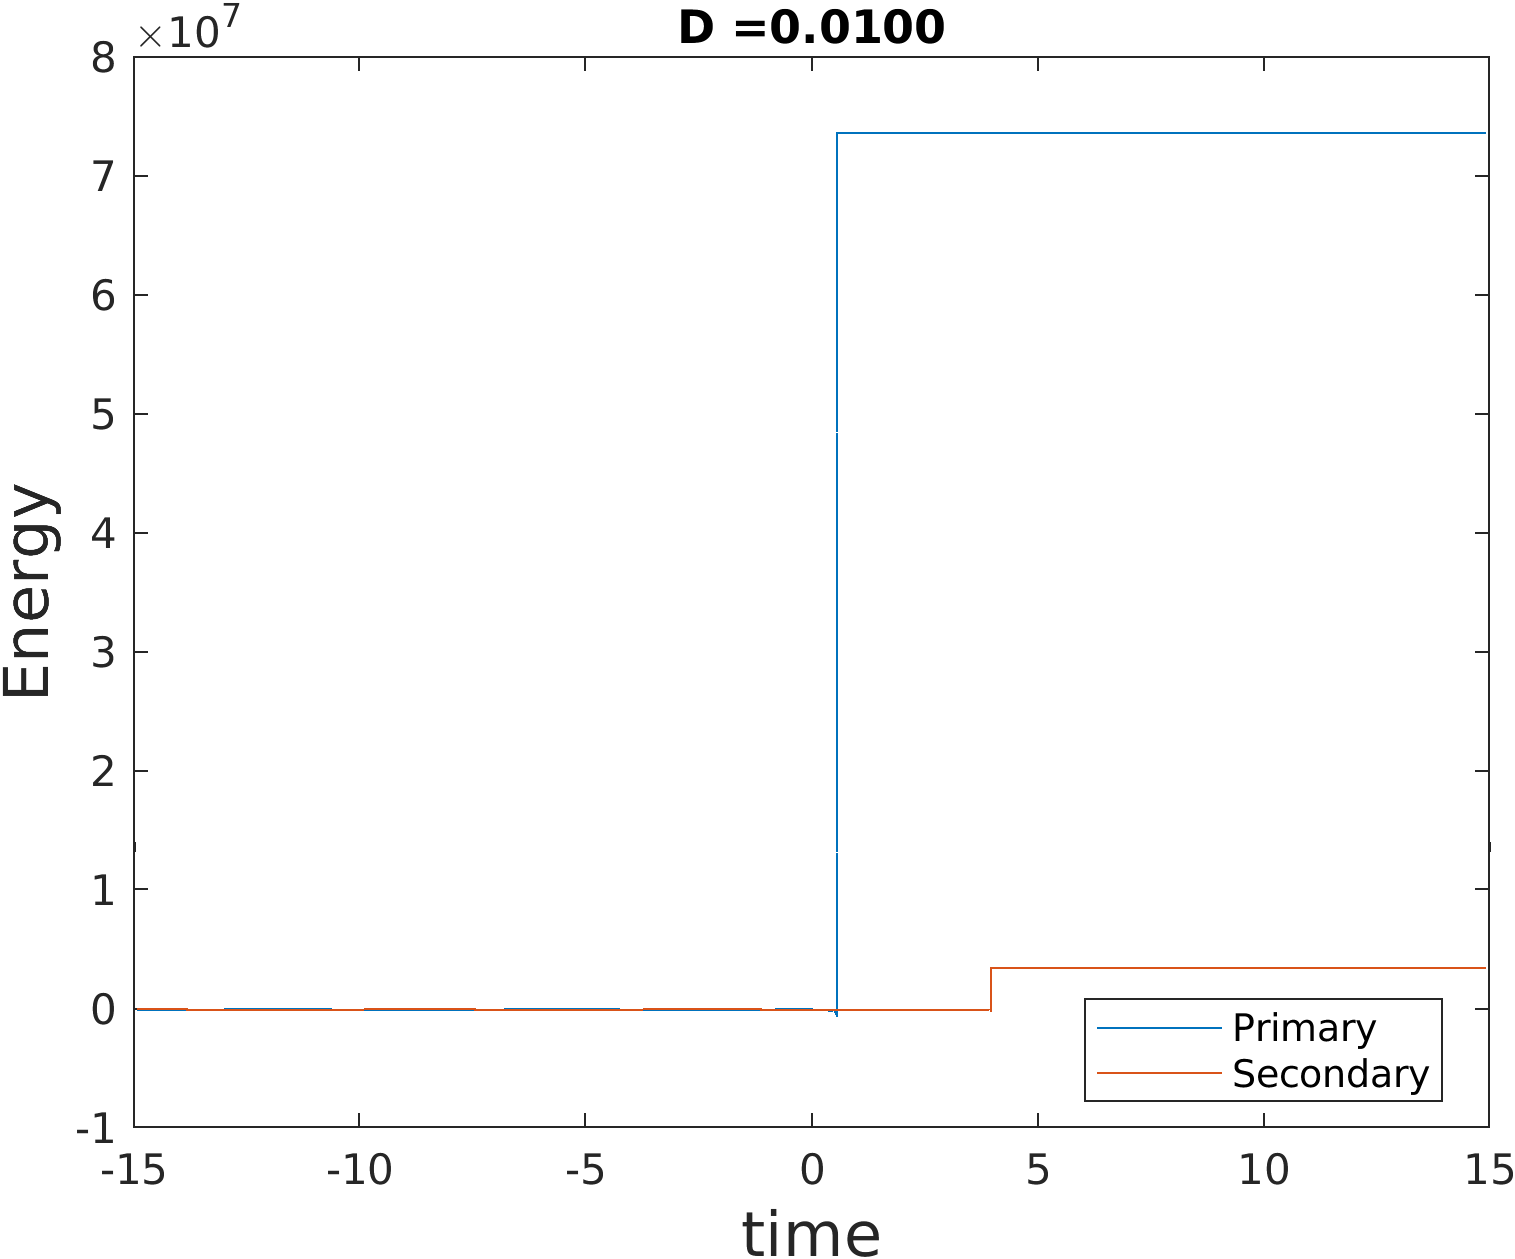
\includegraphics[width=\linewidth, height =.55\linewidth] {../plots/3f/retrograde_energies/1.png}
					\end{subfigure} %
					\hspace{1.7cm}
					\begin{subfigure} {.425\linewidth}
						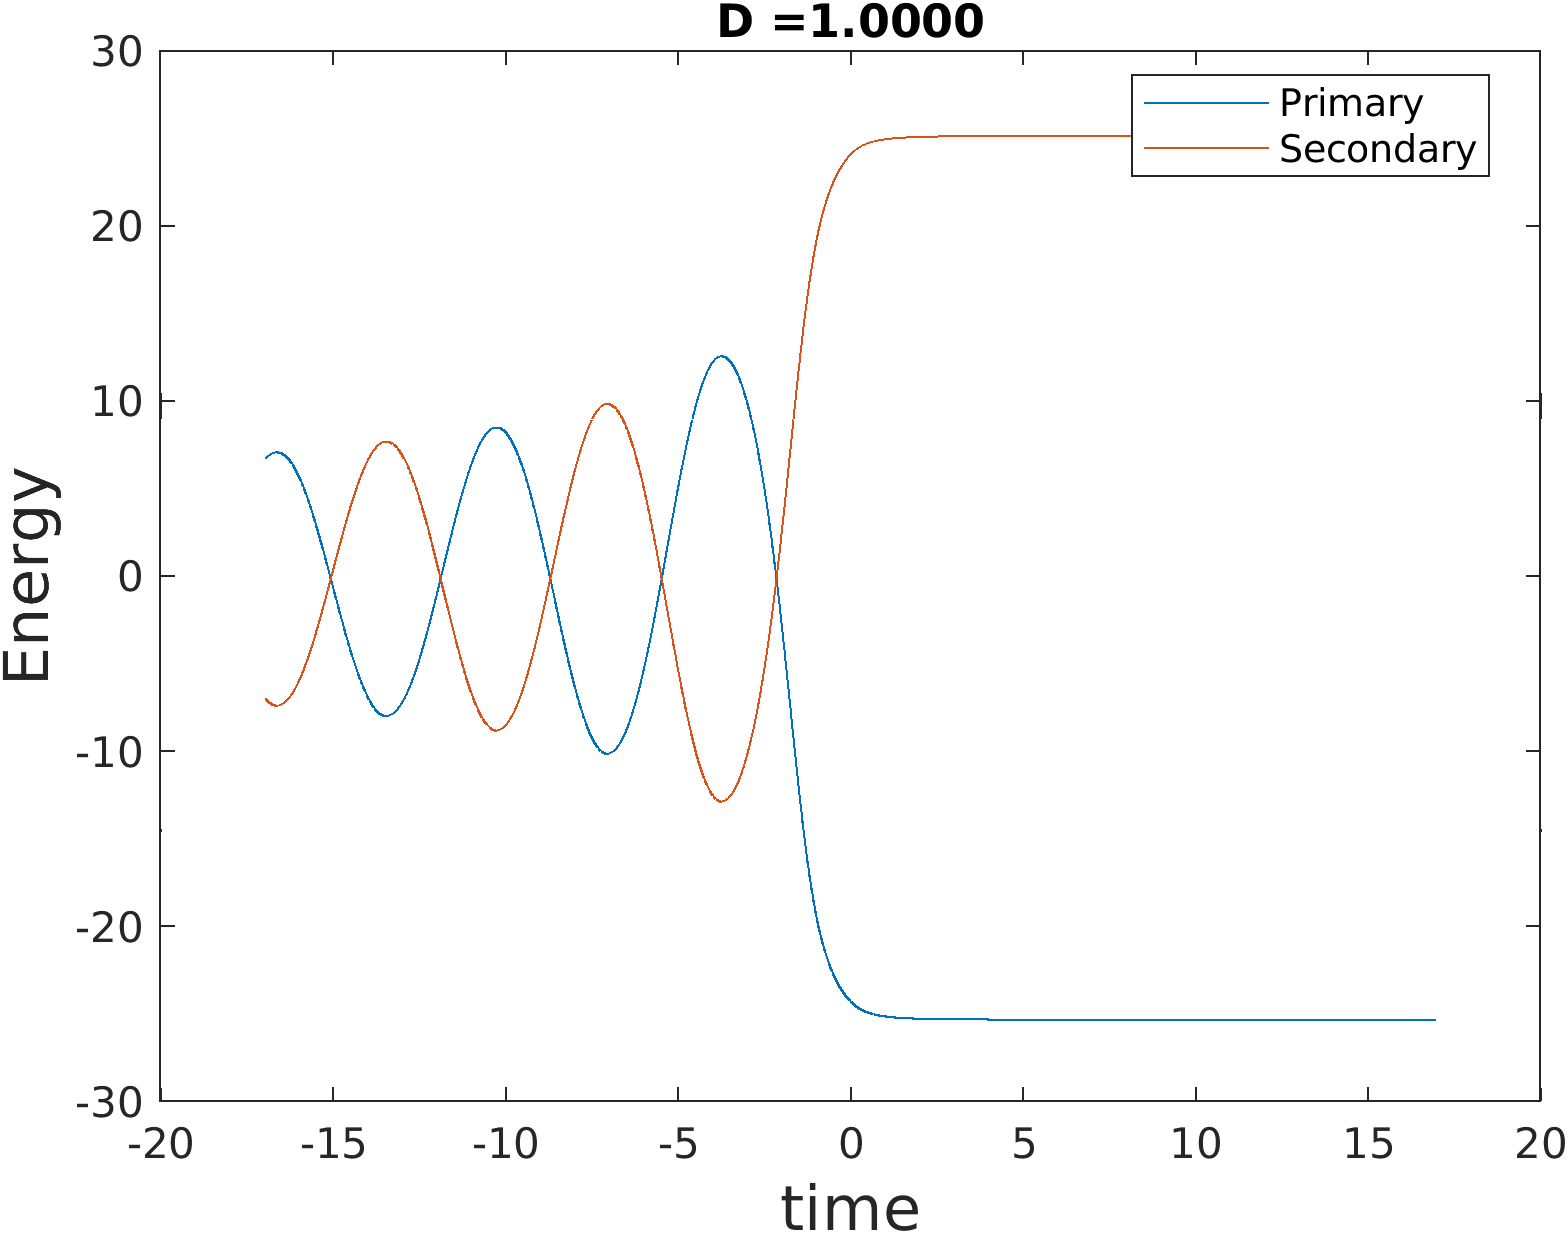
\includegraphics[width=\linewidth, height =.55\linewidth] {../plots/3f/prograde_energies/6.png}\\
						\vspace{1.5mm}
						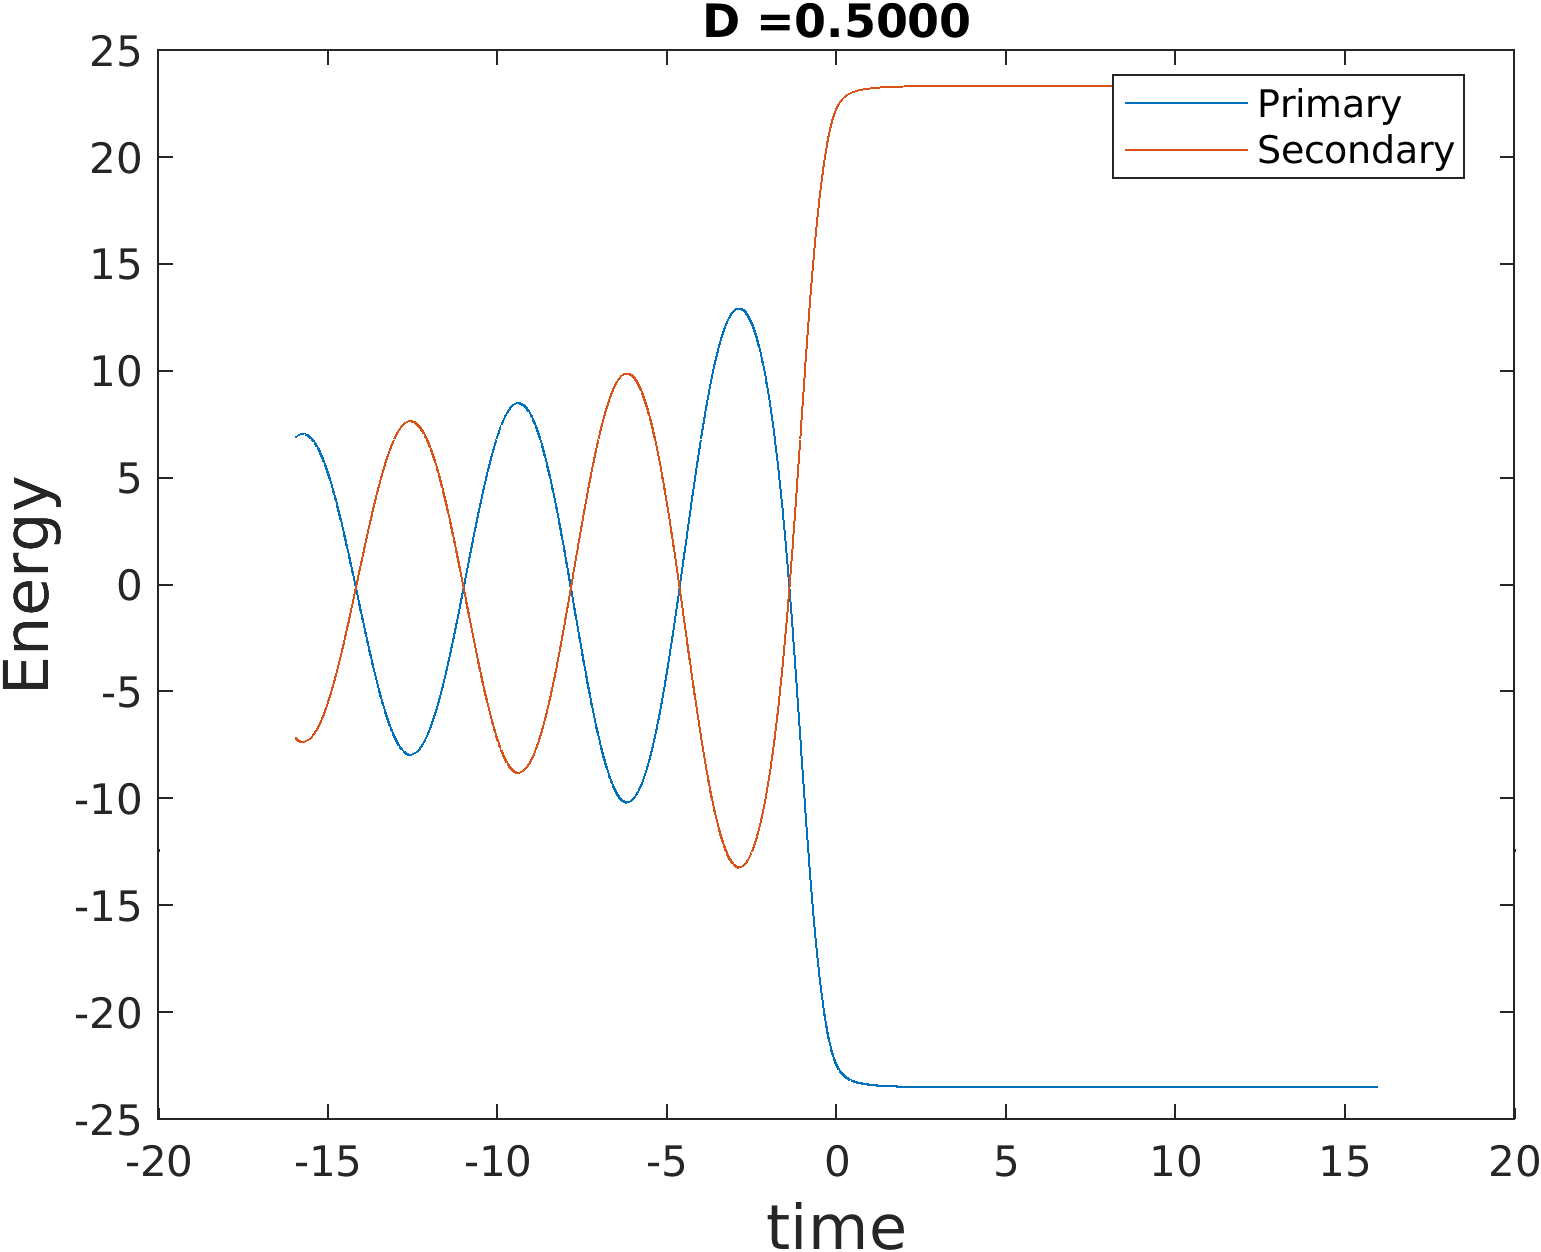
\includegraphics[width=\linewidth, height =.55\linewidth] {../plots/3f/prograde_energies/5.png}\\
						\vspace{1.5mm}
						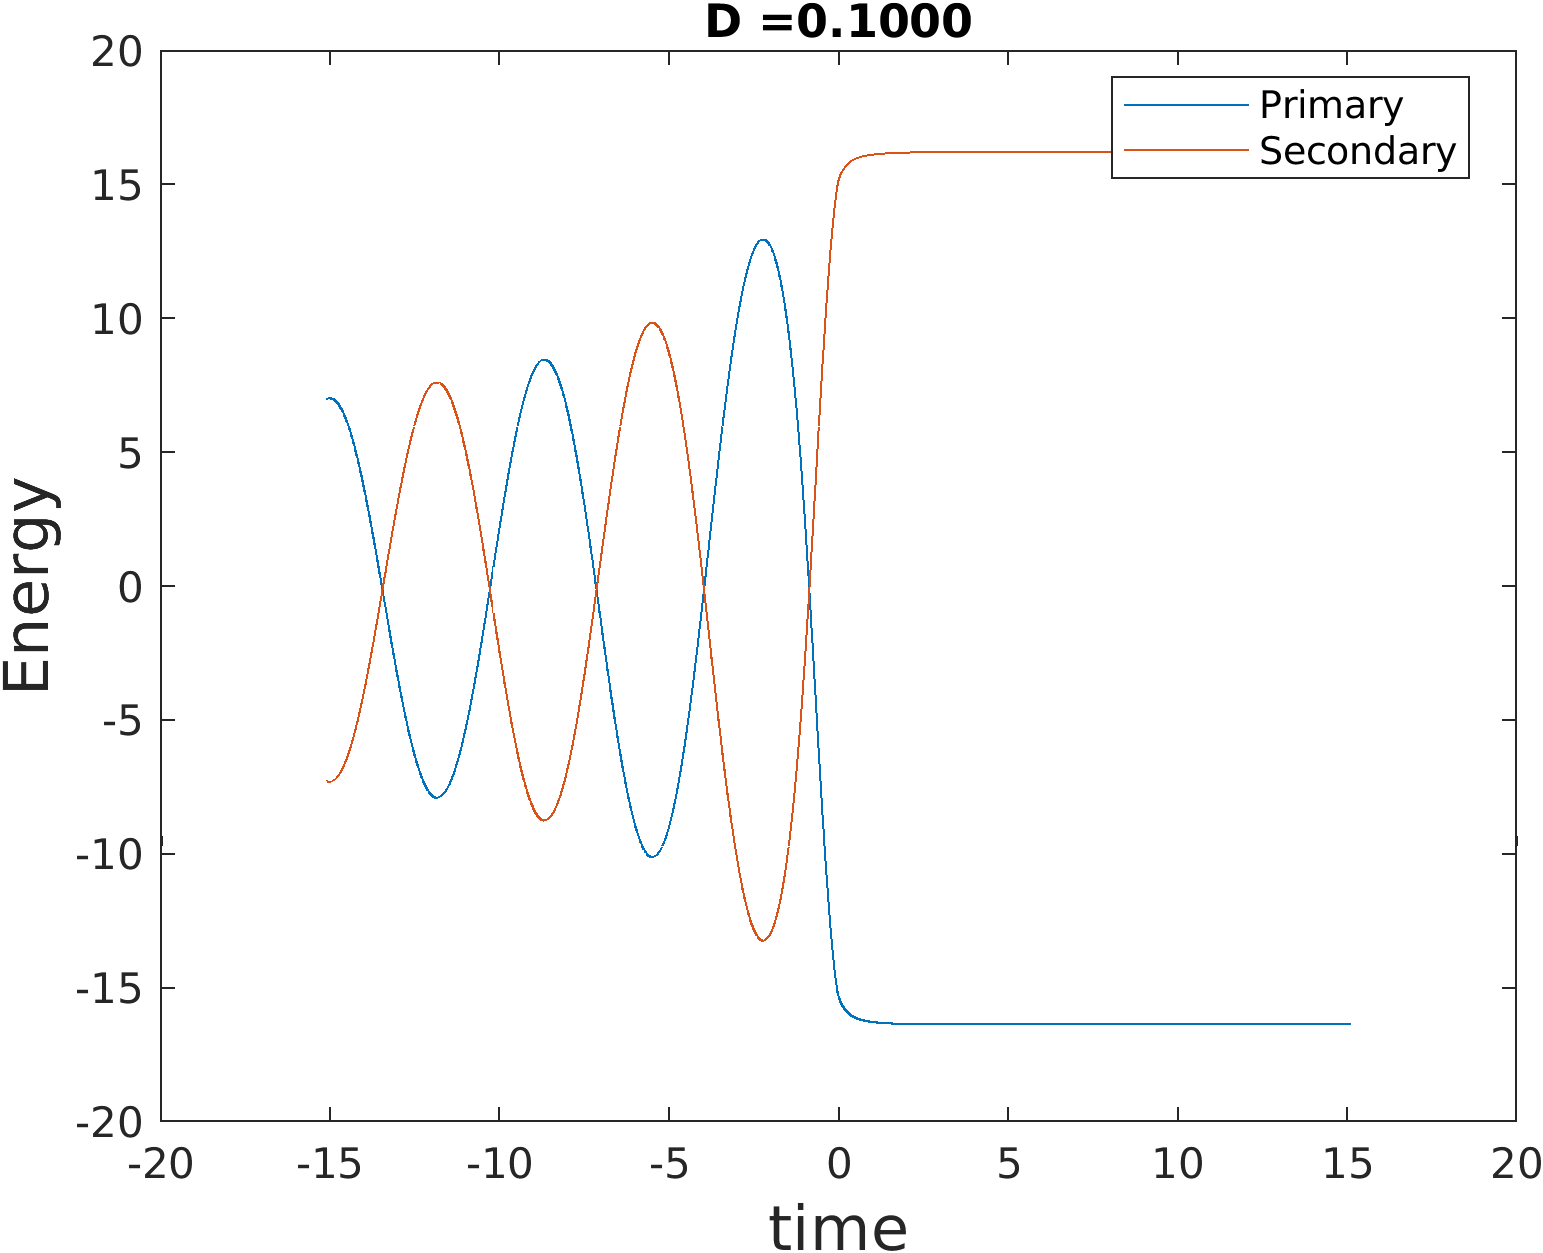
\includegraphics[width=\linewidth, height =.55\linewidth] {../plots/3f/prograde_energies/4.png}\\
						\vspace{1.5mm}
						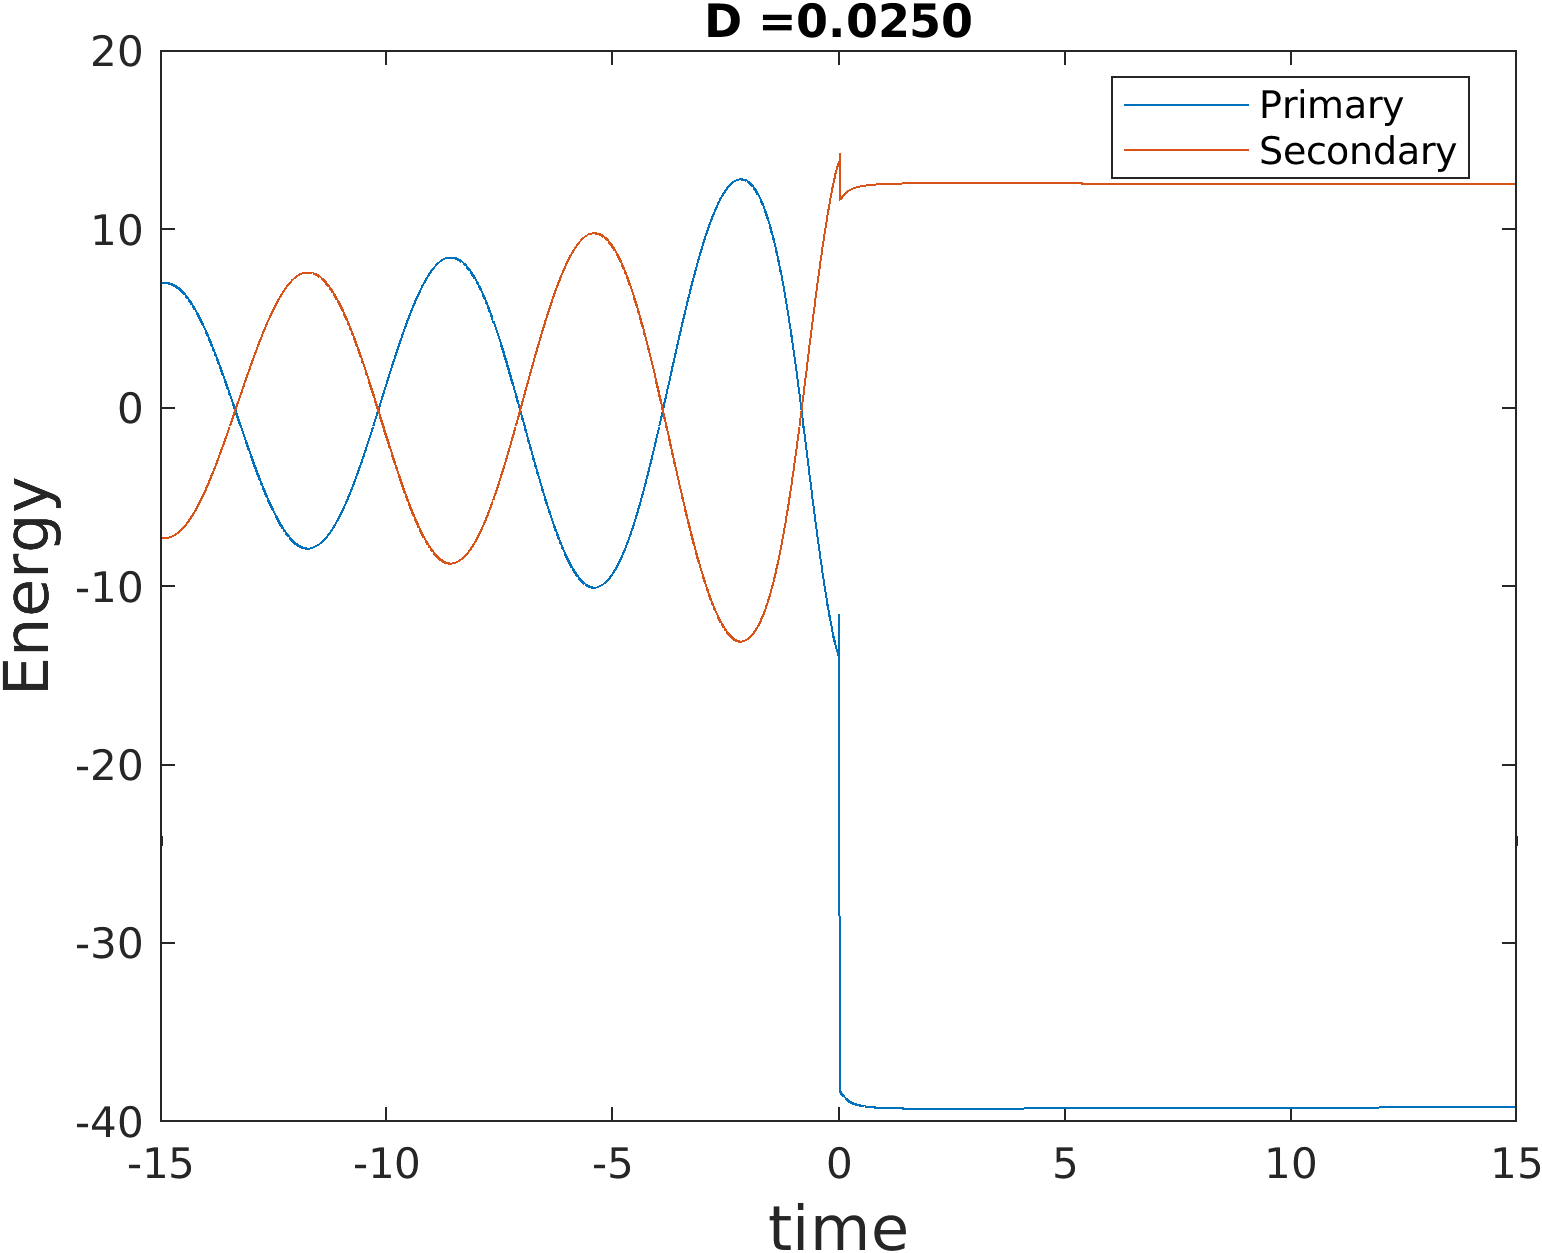
\includegraphics[width=\linewidth, height =.55\linewidth] {../plots/3f/prograde_energies/3.png}\\
						\vspace{1.5mm}
						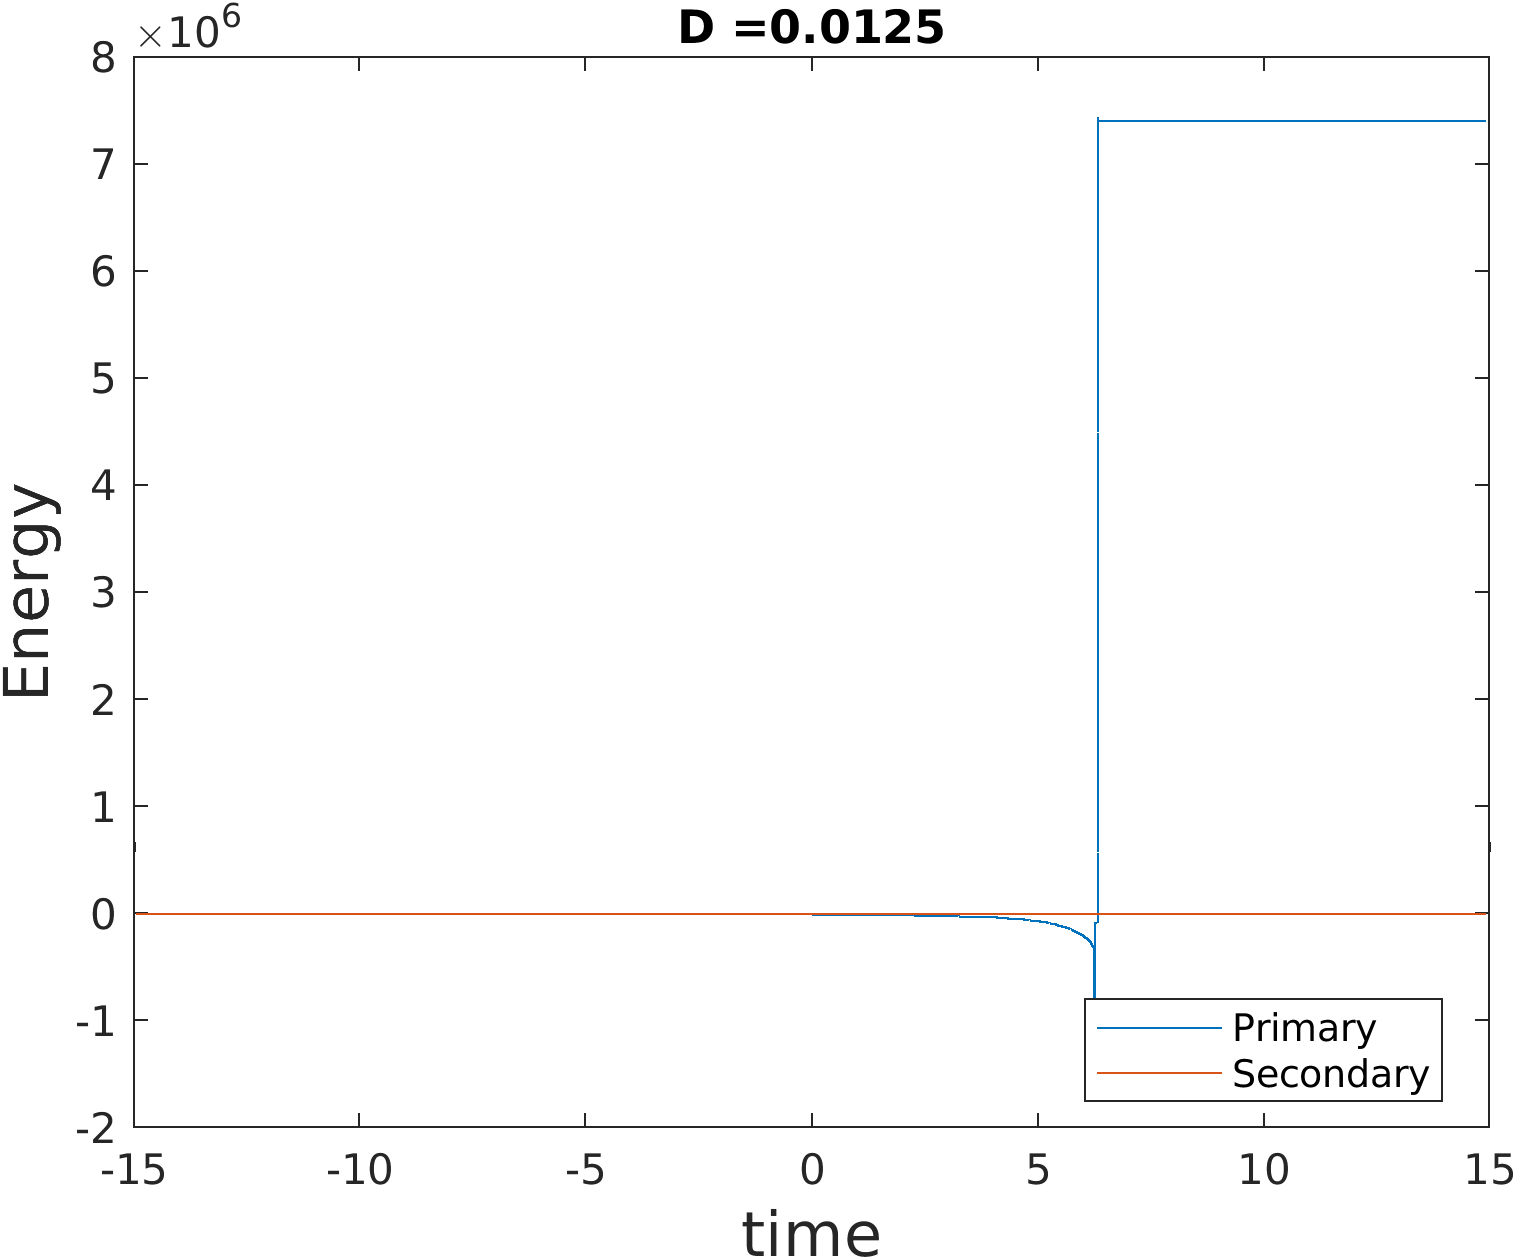
\includegraphics[width=\linewidth, height =.55\linewidth] {../plots/3f/prograde_energies/2.png}\\
						\vspace{1.5mm}
						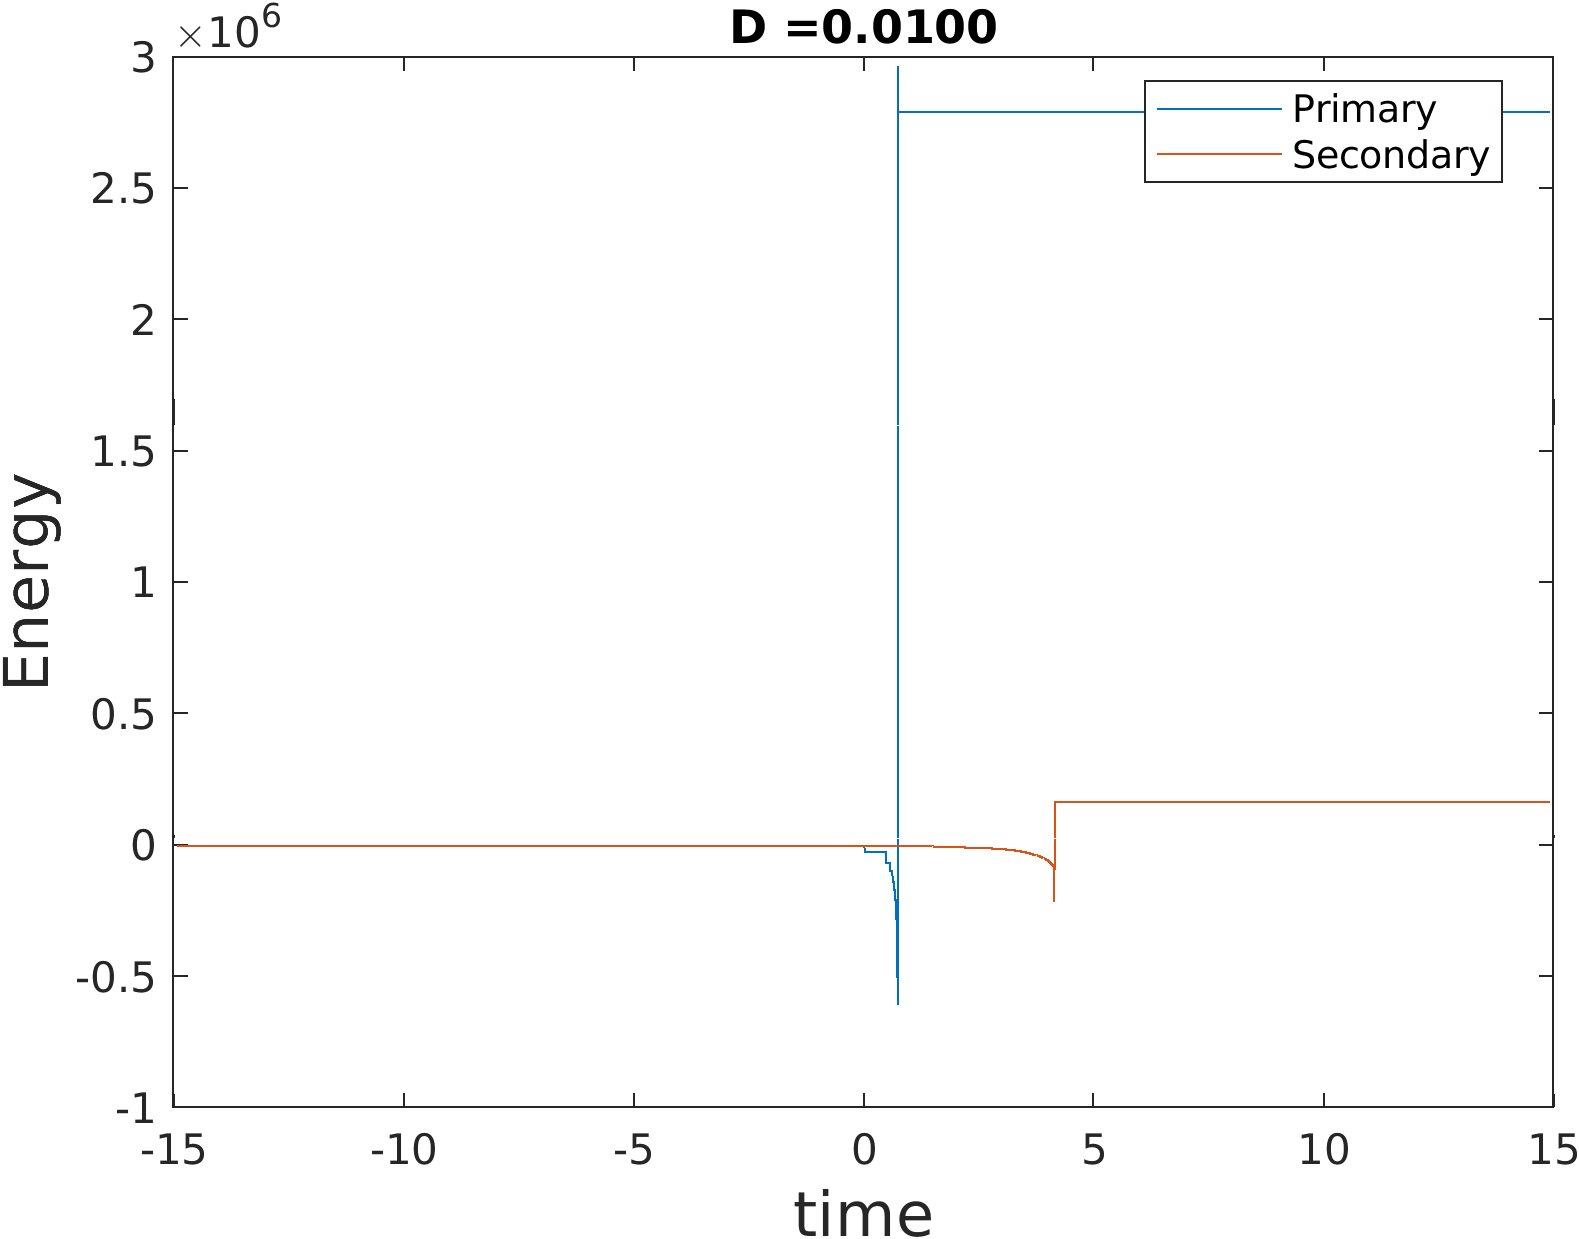
\includegraphics[width=\linewidth, height =.55\linewidth] {../plots/3f/prograde_energies/1.png}
					\end{subfigure}
					\caption{A comparison of evolution of energies of clockwise (left) and counter-clockwise (right) binaries for different values of penetration factor \(D\) = 1.0, 0.5, 0.1, 0.025, 0.0125 and 0.01, for the cases of tidal breakups of binaries. These energies correspond to orbits shown in figure \ref{fig:3f-orbits_pro_retro}.}
					\label{fig:3f-energies_pro_retro}
				\end{figure}
				
				\begin{table}
					\centering
					\begin{tabular} {l r r}
						\toprule
						\textbf{D} & \textbf{Energies (counter-clockwise)} & \textbf{Energies (clockwise)} \\
						\midrule
						1.0 & (-25.2675, 25.1855) & (-0.0890, -0.1091) \\
						0.5 & (-23.4682, 23.3859) & (9.6326, -9.9671) \\
						0.1 & (-16.3085, 16.2244) & (14.6806, -14.7687) \\
						0.025 & (-39.1484, 12.5554) & (-8.3239, -18.3726) \\
						0.0125 & (\(7.4 \times 10^6\) ,\(-4.33 \times 10^2\)) &  (\(6.85 \times 10^5\),\(-4.84 \times 10^2\)) \\
						0.01 & (\(2.79 \times 10^6\),\(1.65 \times 10^5\)) & (\(7.36 \times 10^7\)  ,\(3.52 \times 10^6\)) \\
						\bottomrule
					\end{tabular}
					\caption{Final energies of two stars (primary, secondary) in the simulations of binaries for different values of penetration factor, \(D\).}
					\label{table:3f-final_energies_d}
				\end{table}
				
				\subitem \textbf{Results --}
				The orbital trajectories obtained for different values of \(D\), for clockwise and counter-clockwise rotating binaries is shown in figure \ref{fig:3f-orbits_pro_retro}. Corresponding binary energy evolutions are shown in figure \ref{fig:3f-energies_pro_retro}. The final value of energies of primary and secondary stars is enlisted in table \ref{table:3f-final_energies_d}
				
				\subitem \textbf{Discussions --}
				Figure \ref{fig:3f-orbits_pro_retro} clearly demonstrates that clockwise rotating binaries are more stable to tidal disruption than counter-clockwise rotating binaries. This can be seen most prominently for cases \(D=1.0\text{ -- }0.1\).
				In the energy evolution plots of figure \ref{fig:3f-energies_pro_retro}, these effects are most pronounced for \(D=1.0\text{ and }0.5\).
				
				The extreme case tidal disruptions are essentially similar for both cases with both stars getting ejected, as seen for \(D=0.01\). One another possibility for such close interactions is the complete disruption and \emph{swallow up} of the binary by the super massive black hole. On the other hand, in somewhat less extreme cases, such as for \(D=0.0125\), one of the stars is captured in highly eccentric orbit while the other one is ejected at extremely high speed.
				
				For the case of \(D=0.1\) considered in previous section in equation \ref{eq:3-velocity_at_inf}, if we consider the final energy obtained in table \ref{table:3f-final_energies_d}, the value of velocity at \(r=\infty\) for clockwise rotating binary turns out to approximately 3998 km/s instead of approximately 4200 km/s obtained for counter-clockwise rotating binary.
				
				From these observations, it can be safely concluded that orientation of rotation of binary has a profound impact on evolution of the system in the vicinity of black hole.
				
					
			\end{enumerate}


		% -------------------------------- Conclusions --------------------------------------

		\clearpage
		\section{Conclusions} \label{3:conclusions}
		Binary star systems around super massive black holes get tidally disrupted in case the distance of closest approach is less than some threshold value. If the distance of closest approach is less than that value, one star of the binary get more strongly bound in a tighter lower energy orbit while the other one flies off in a higher energy trajectory. This phenomenon results in occurrence of hyper velocity stars. In extreme cases of very close approaches, the stars may get tidally destroyed by the black hole's gravity, thereby becoming sources of observable transient tidal disruption flares.
		

\end{document}